\chapter{Signal Systematics}
\label{chap:systematics}

In order to use this analysis to make a statement about a potential \ac{BSM} model, the extent to which the signal \ac{MC} correctly simulates the real physical environment must be evaluated. Differences between data and \ac{MC} are studied in order to avoid underestimating or overestimating the expected number of \ac{BSM} events that could have been seen in the data.

Where possible, the \ac{MC} is corrected to better represent the data using \emph{scale factors}, and in other cases systematic uncertainties are applied to the final result. Uncertainties are also evaluated on the scale factors. A list of all of the systematic uncertainties applied in the interpretation are listed in \autoref{tab:siguncertainties}. The value listed in the table describes how much varying the efficiency of a given parameter changes the final signal yield. 

The dominant source of systematic uncertainty on the signal \ac{MC} in this analysis comes from the efficiency for selecting displaced leptons, for which there is no data to compare to \ac{MC}. As a result, this is evaluated in several steps: first the trigger, reconstruction, and selection efficiencies are compared for prompt leptons in the same physics process in data and \ac{MC}; then the tracking efficiency is compared between signal muons and cosmic muons, which compares different physical phenomena that result in \pt, high \absdz tracks; finally, the lepton reconstruction efficiency is studied with respect to displacement is studied in \ac{MC} only and a conservative additional uncertainty to account for any missed effects in data is measured. Other event-level systematic uncertainties are applied to account for mismodeling of pileup and theory assumptions made during \ac{MC} generation. There are many standard systematic uncertainties derived by \ac{ATLAS}, for example the jet energy measurements or the sagitta measurements of muons, that do not have a large impact on this analysis with its nonstandard physics objects.

\begin{table}[htb]
\small
\begin{center}
\begin{tabular}{lcc}
Uncertainty Source & Uncertainty [\%] (\selec/\smu)  &  Uncertainty [\%] (\stau)  \\
\hline
Statistical				& 2-46    & 2-100                 \\
Cross Section 			& 2-5     & 2-5                 \\
Tracking				& 2-15    & 11-14                 \\
Muon Trigger			& 1-4     & 4            \\
Muon Selection	        & 3-15    & 20-37          \\
Electron Selection      & 0.5-2   & 1-2    \\
Electron Trigger	    & 0       & 0       \\
Lepton Displacement  	& 1-18    & 2-26         \\
Pileup Modeling     	& 7       & 7            \\
Other theory         	& 0-5     & 0-5              \\
\texttt{DRAW\_RPVLL} Filter Efficiency		& 1.5     & 1.5          \\
Luminosity				& 2       & 2          \\
\hline
\end{tabular}
\caption{Table describing statistical and systematic uncertainties impacting \selec, \smu and \stau efficiencies. Systematics in this table are defined as the difference varying each parameter makes in the final signal yield.} 
\label{tab:siguncertainties}
\end{center}
\end{table}


\section{Displaced Lepton Reconstruction}

\subsection{Prompt Lepton Reconstruction}
Z bosons can decay into two electrons or two muons. This process is well modeled in \ac{MC}, and easy to identify in data as the invariant mass of the two leptons should equal the Z boson mass (within resolution effects). The invariant mass of the leptons provides a way to identify a lepton as a real lepton that should pass all of the trigger, reconstruction, identification, and selection algorithms. A \emph{tag-and-probe} analysis \emph{tags} events by finding two lepton candidates with invariant mass near the Z boson peak, and then the \emph{probe} leptons are used to measure the selection efficiency by asking that one of the leptons pass a given requirement. This method is used to evaluate trigger, reconstruction, and selection efficiencies of prompt electrons and muons.

The difference between data and \ac{MC} can be thoroughly studied, so scale factors are applied to correct the leptons in MC. A scale factor is defined as:

\begin{equation}
\text{scale factor} = \frac{\text{efficiency in data}}{\text{efficiency in MC}}
\end{equation}
Then the statistical uncertainty on this value is evaluated and applied as an additional uncertainty on the signal. In general, \ac{MC} estimates higher efficiencies than are seen in data. In particular, the \ac{MC} assumes a perfectly aligned detector with all subsystems working perfectly, which is not true in practice, so variables that correlate multiple subdetectors, like electron \dpt or muon \chiCB, contribute to a difference between data and \ac{MC}. A 90\% scale factor means that \ac{MC} overestimates the selection efficiency by 10\%.   

\ac{ATLAS} centrally defines electron and muon scale factors for prompt electrons and muons, but due to the special triggers and selection criteria used in this analysis, custom scale factors are required. For electrons, this analysis uses photon triggers as well as a bug-fixed electron reconstruction, as well as a custom identification and non-standard selection criteria, so all scale factors must be derived specifically for this analysis. For muons, a nonstandard trigger is used, but the reconstruction is standard (except for the tracking, evaluated separately) and the only change to the identification criteria is the removal of the cut on pixel hits, which does not impact prompt muons, so central scale factors are used, with additional selection and special trigger scale factors derived for this analysis.

\question{I never talked about the electron bug.. i assume that's fine?}

\subsubsection{Electrons}

For electrons, $Z\rightarrow ee$ events are used to evaluate trigger scale factors, and a single scale factor for reconstruction, identification, and selection as all electrons coming from the Z are real electrons and should pass the trigger as well as all selection criteria.

For both \texttt{HLT\_2g50\_loose} and \texttt{HLT\_g140\_loose} triggers, the efficiency is defined as the number of electrons passing the trigger divided by the number of electrons passing the offline identification criteria. This is done for single electrons, and in the case of the 2 electron trigger, the results are summed in quadrature. It was found that above the trigger threshold, the trigger efficiency in both data and \ac{MC} is very close to 100\%, so this scale factor and its associated uncertainty is considered negligible.

The reconstruction, identification, and selection scale factors are evaluated together, by measuring the efficiency for a reconstructed electron candidate to pass the final signal selection. Electron candidates are cluster-track combinations that will get eventually identified as a photon, converted photon, or electron (or none of these). The track reconstruction is studied separately and the cluster reconstruction efficiency at the signal \pt is nearly 100\%. The scale factors for electron selection are defined as a function of $E_{T}$ and $\eta$ and around 98\% except for in the region between the barrel and endcap (around $|\eta|$ = 1.5) where it drops to 90\%. The statistical uncertainty varies from 1-3\%. 


\subsubsection{Muons}
$Z\rightarrow \mu\mu$ data and \ac{MC} are used to define additional scale factors for the \texttt{HLT\_mu60\_0eta105\_msonly} trigger. The standard trigger scale factors correct for many features of the \ac{MS} and additional corrections are derived and applied on top of them for this analysis. Events are required to pass a \ac{MET} trigger to ensure an unbiased data sample and have two muons within 10 GeV of the mass of the Z boson. The trigger efficiency is then defined as the number of muons passing the \texttt{HLT\_mu60\_0eta105\_msonly} trigger divided by the number of baseline muons. Similarly, selection scale factors are defined by requiring that one muon pass all signal selections (except the \absdz cut), then the efficiency for the second baseline muon to pass the same signal selection cuts is evaluated.

The scale factors are larger for muons than for electrons because many of the structural features of the \ac{MS} are not well modeled in \ac{MC}. The statistical errors are also around 3\%.


\subsection{Tracking}

This analysis relies on \ac{LRT} in order to reconstruct leptons with high \pt and high \absdz. 
Tracks from cosmic muons have high \pt and high \absdz and can be used to measure the tracking efficiency in data. Cosmic muons are tagged as muons with \ac{MS} activity on the other side of the detector, so the cosmic muon must have also passed through the \ac{ID} leaving a track behind. Provided we make some kinematic selections, the existence of the track back-to-back with the cosmic should be solely dependent on the \ac{LRT} efficiency.

A tag-and-probe analysis is performed here as well, by tagging a cosmic muon and looking for tracks back-to-back with it in a narrow $\Delta R_{\text{cos}}$ cone. Then compare this to a tag-and-probe analysis in signal \ac{MC} by looking for a track in a narrow $\Delta R$ cone nearby a truth muon. 

There are several important kinematic selections that must be made to ensure the collection of tracks are similar and to correct for the different kinematic distributions between cosmics and data (see \autoref{fig:cos_eff}). 

First, to ensure all the hits in the track will be read out with the event, $\phi > 0$ muons must have negative \tavg (early w.r.t collision), and $\phi < 0$ muons must have positive \tavg (late w.r.t collision). Making this cut shows a flat reconstruction efficiency w.r.t. \tavg. All signal muons have very central timing, with \ac{ID} signatures created before \ac{MS} signatures, so this problem does not apply. The impact of the timing cut can be seen in \autoref{fig:cos_sys_t0}. 

Second, the cosmic ray muon passes through the detector in an approximately straight line through the \ac{ID}, so the \dz is simply the distance the cosmic muon was from the PV. This is not the case for signal muons, whose \dz does not measure a point the muon has gone through, but an extrapolation backwards to the PV. This means that signal tracks with the same \dz can have very different properties, such as number of hits on track. To correct for this, we require the $R_{\textrm{decay}}$ and \dz to fall between the same two silicon layers. A sketch of this difference can be seen in \autoref{fig:lrt_sig_sketch}. 

Finally, cosmic muons have a much wider \z range than signal muons, which induces an $\eta$ dependence. So we require cosmic muons to have $\absz < 120$ mm, to harmonize with signal muons. Additionally, both signal and cosmic muons must have $|\eta| < 1.05$ in order to be triggered. A full list of cuts made on tag muons and probe tracks can be found in \autoref{tab:lrt-mu-cuts} and \autoref{tab:lrt-track-cuts}.

The remaining difference between cosmic and signal muons is the correlation between \pt and \absdz in signal. Thus, the cosmic muon \pt distribution is reweighted in each \absdz bin to match the signal distribution. Then, the ratio of the efficiencies as a function of \absdz is determined per lepton. The maximum difference, 8\%, is taken as the systematic uncertainty per lepton, then summed in quadrature for the two leptons in the event resulting an 11\% event-level systematic. Tracking efficiency is assumed to be symmetric around the detector and that after GSF tracking, electron tracking and muon tracking have equivalent efficiency, motivated by \autoref{fig:trk_el_mu}. 



\begin{figure}[htbp]
\centering
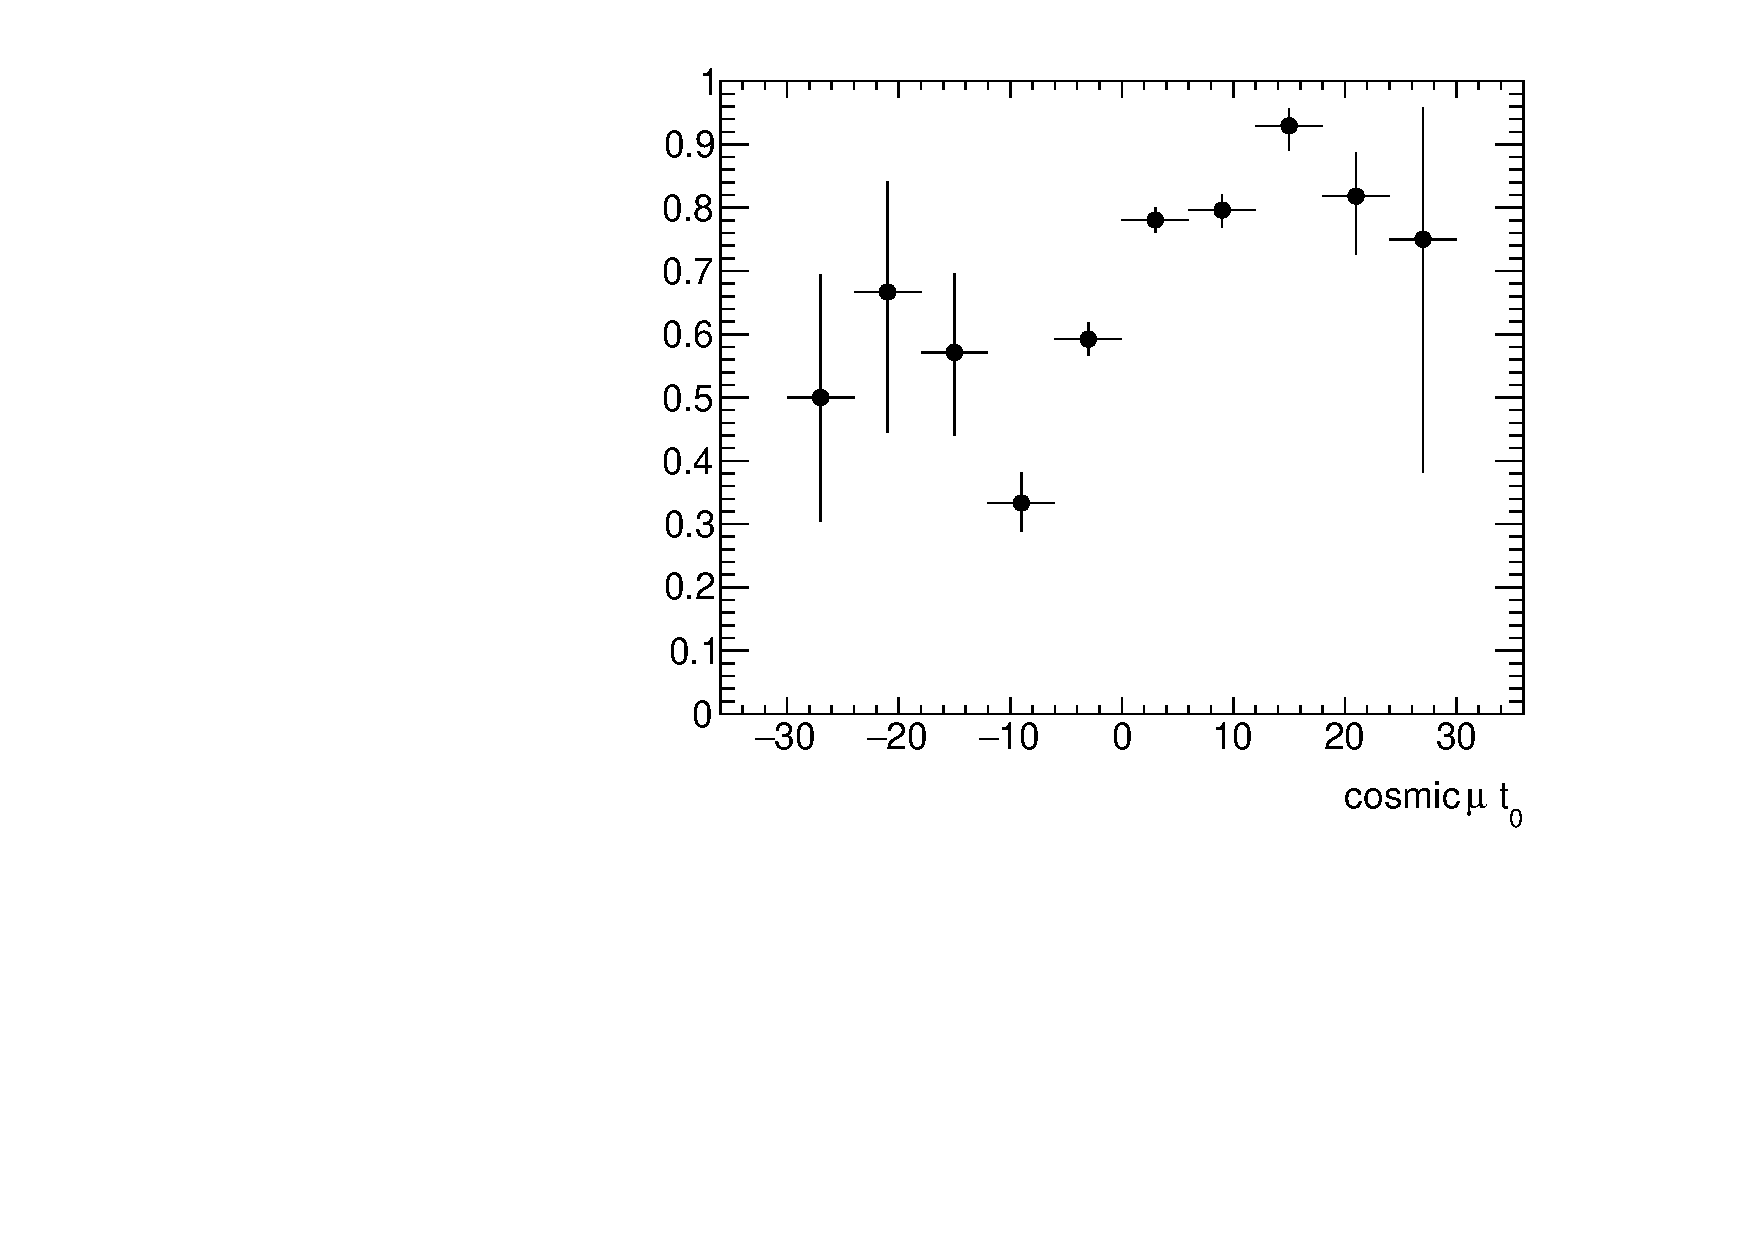
\includegraphics[width=.3\textwidth]{figures/LRT_systs/cosmics_phil0_eff_t0.pdf}
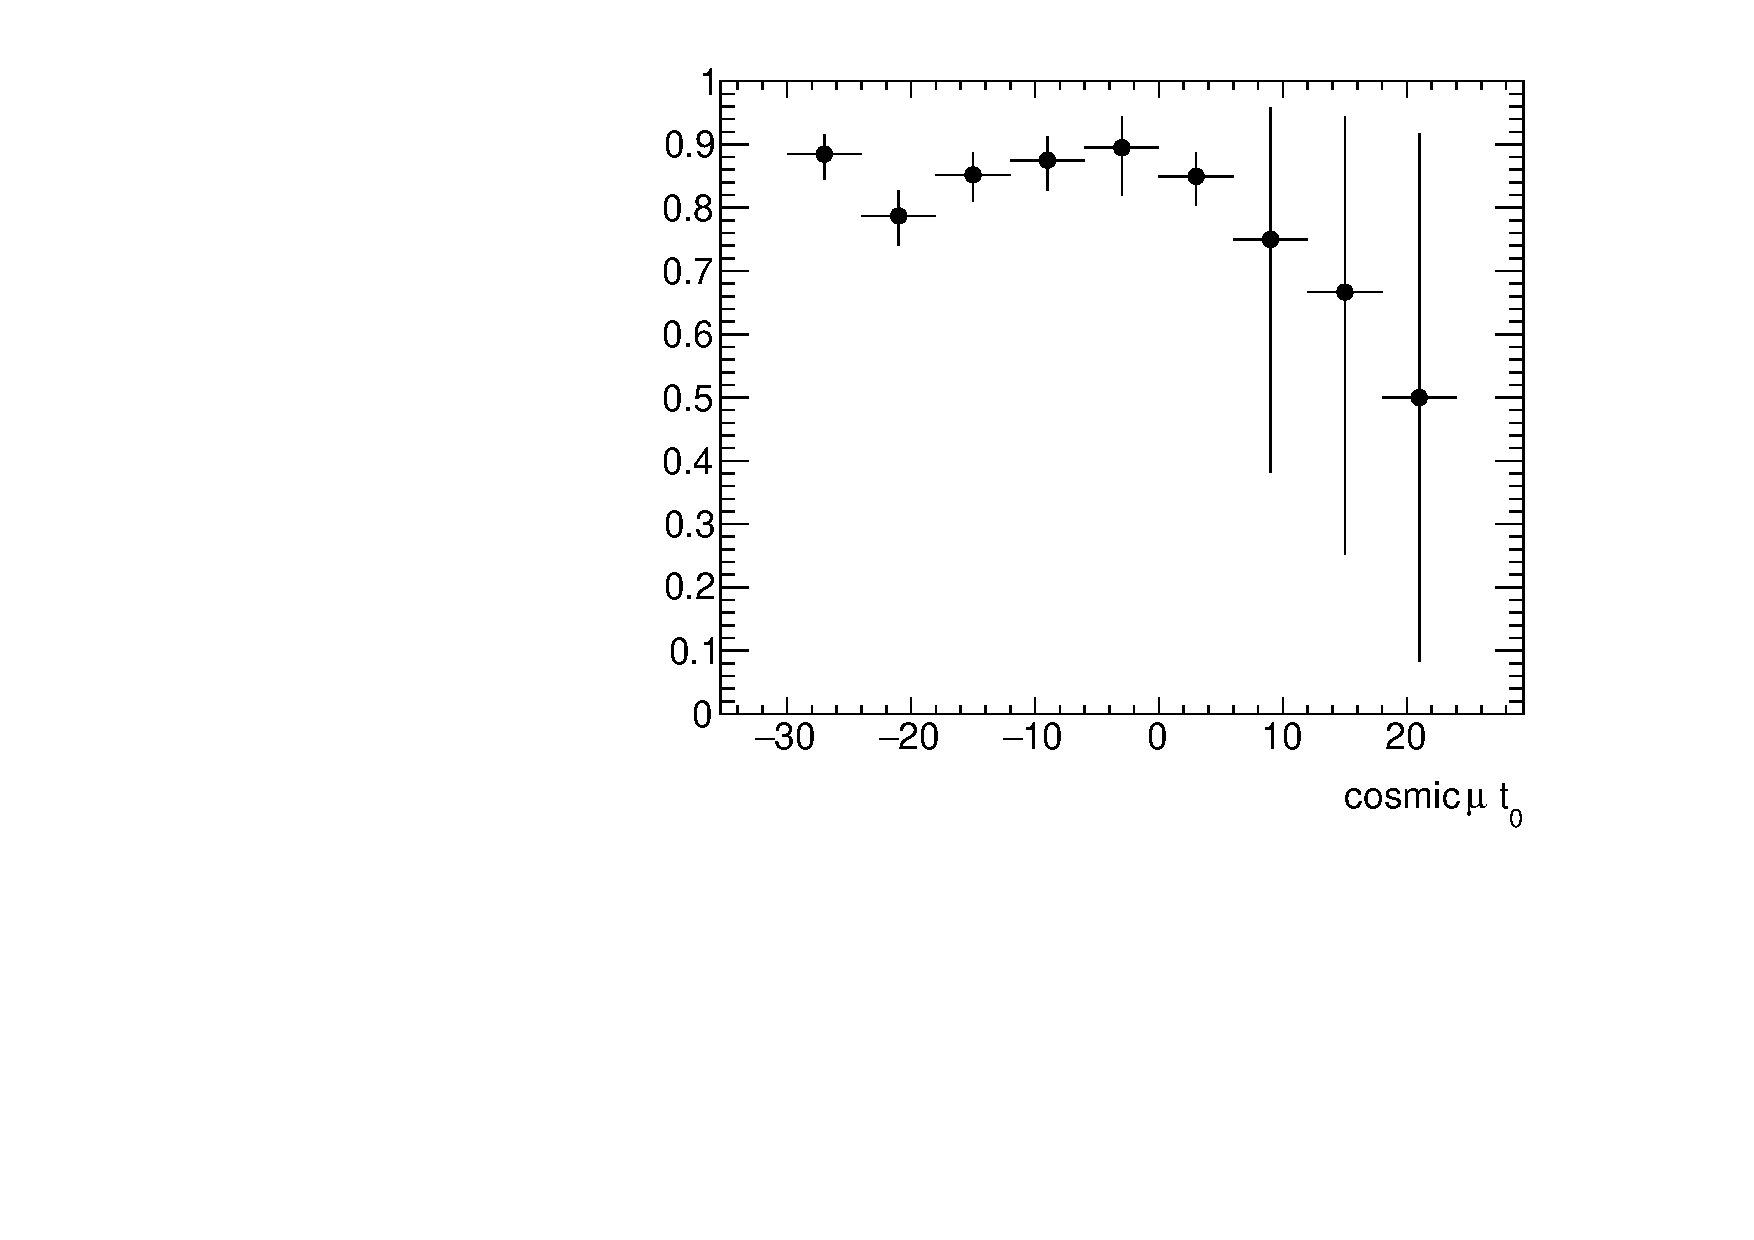
\includegraphics[width=.3\textwidth]{figures/LRT_systs/cosmics_phig0_eff_t0.pdf}
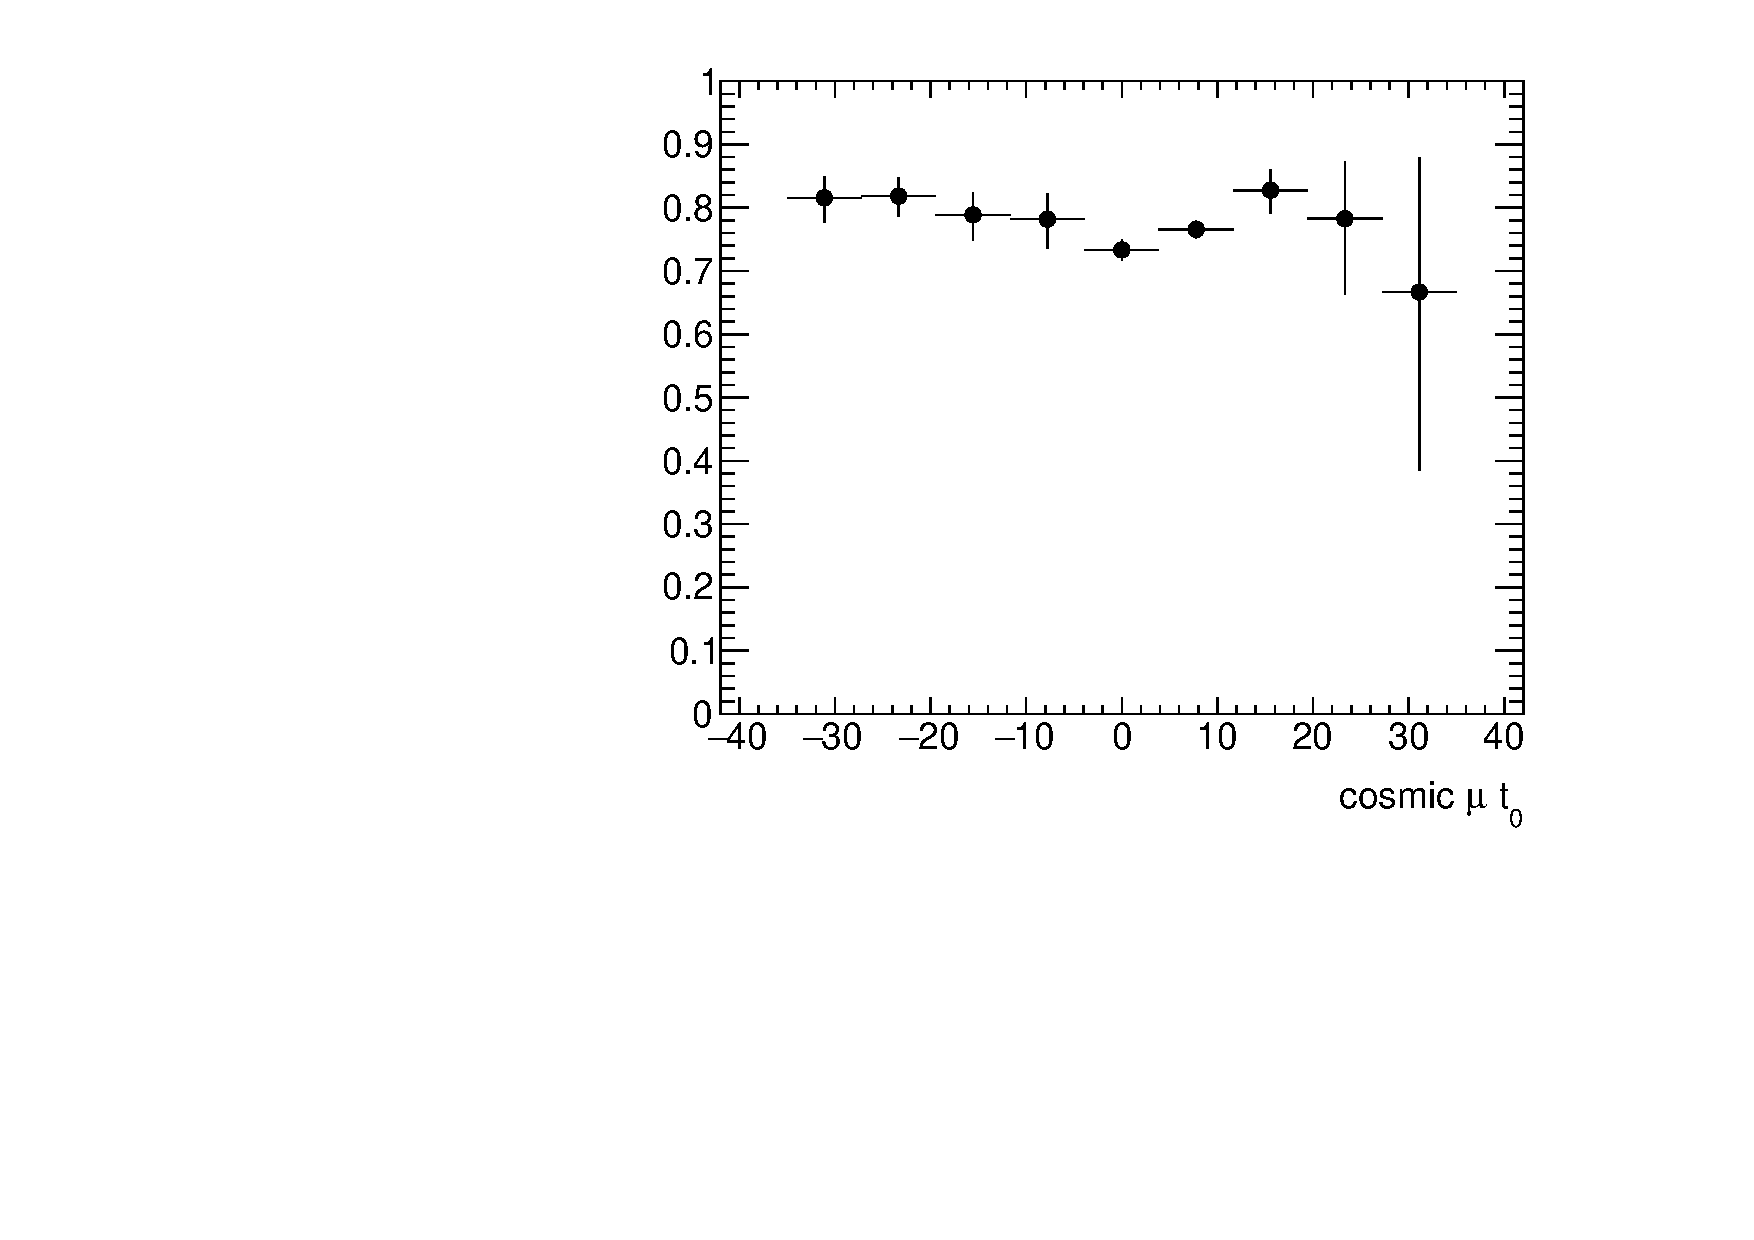
\includegraphics[width=.3\textwidth]{figures/LRT_systs/cosmics_eff_t0.pdf}
\caption{\ac{LRT} efficiency measured with various $\phi$ and \tavg cuts. The right shows $\phi < 0$ muons with no \tavg cut, the center shows $\phi > 0$ muons with no \tavg cut, and the left shows the final selections, with $\phi > 0$ requried to have \tavg < 0 and $\phi < 0$ \tavg > 0. This gives a consistent readout configuration and an approximately flat efficiency w.r.t \tavg. In particular, there $\phi < 0$ muons with negative timing that result in an artificially low efficiency, likely due to incomplete readout.}
\label{fig:cos_sys_t0}
\end{figure}


\begin{figure}[htbp]
\centering
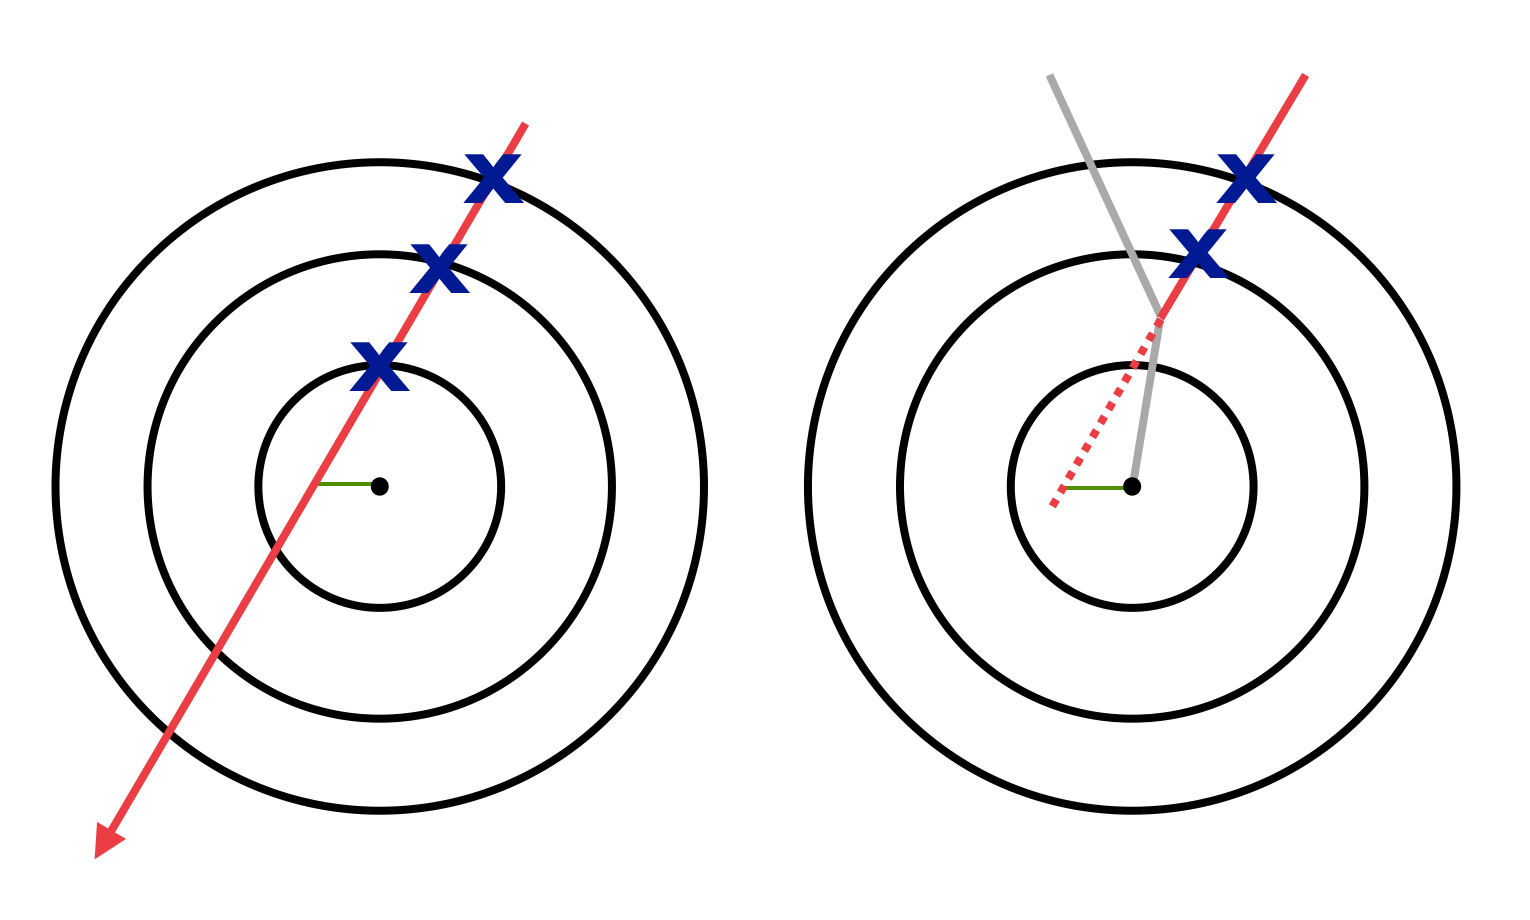
\includegraphics[width=.6\textwidth]{figures/LRT_systs/cos_sig_LRT.png}
\caption{An illustration of the difference in \dz measurements between cosmic (left) and signal muons. The \dz of a cosmic muon is always measured just before its first hit, whereas for a signal muon, the first hit can come far after the \dz. The blue x's represent \ac{ID} hits and the red lines represent muon tracks.}
\label{fig:lrt_sig_sketch}
\end{figure}


\begin{figure}[htbp]
\centering
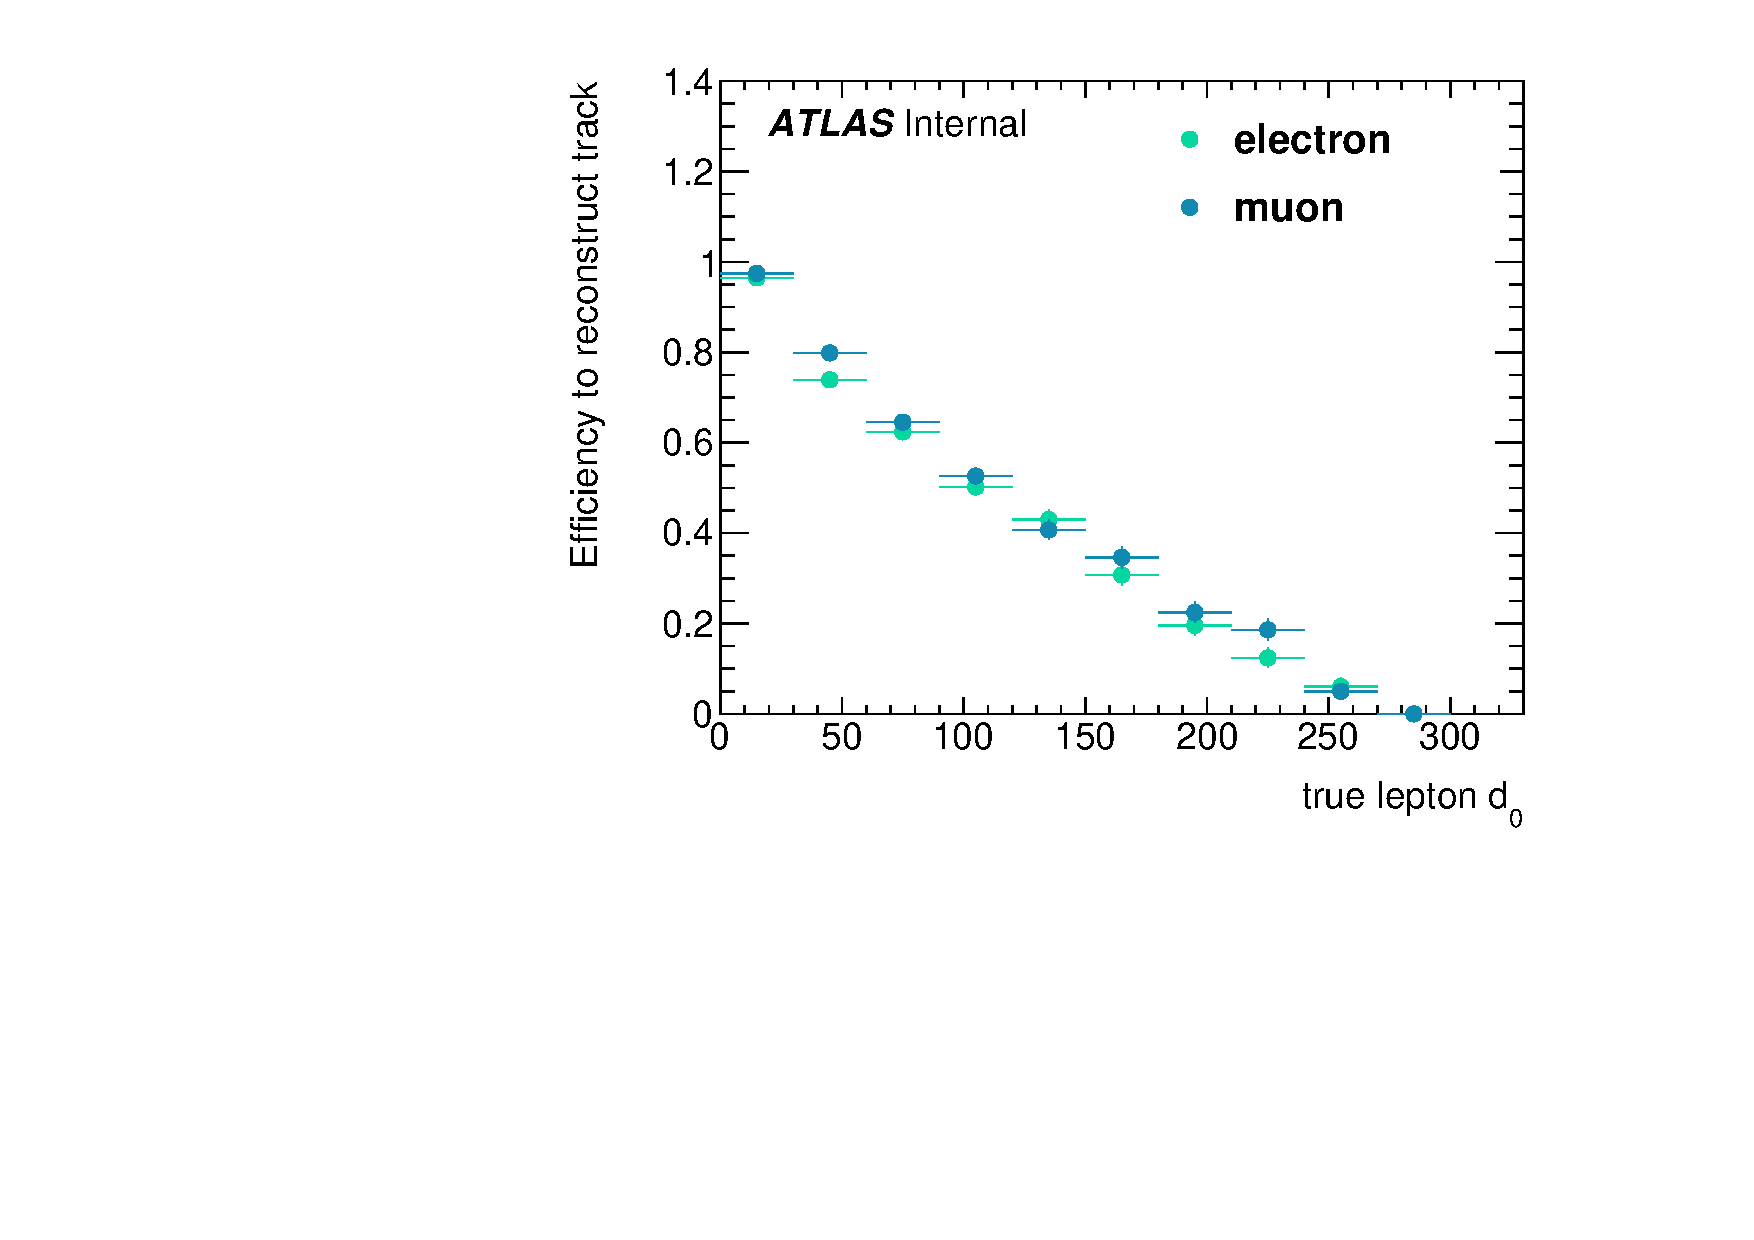
\includegraphics[width=.48\textwidth]{figures/LRT_systs/stlrt_compare_elmu_d0.pdf}
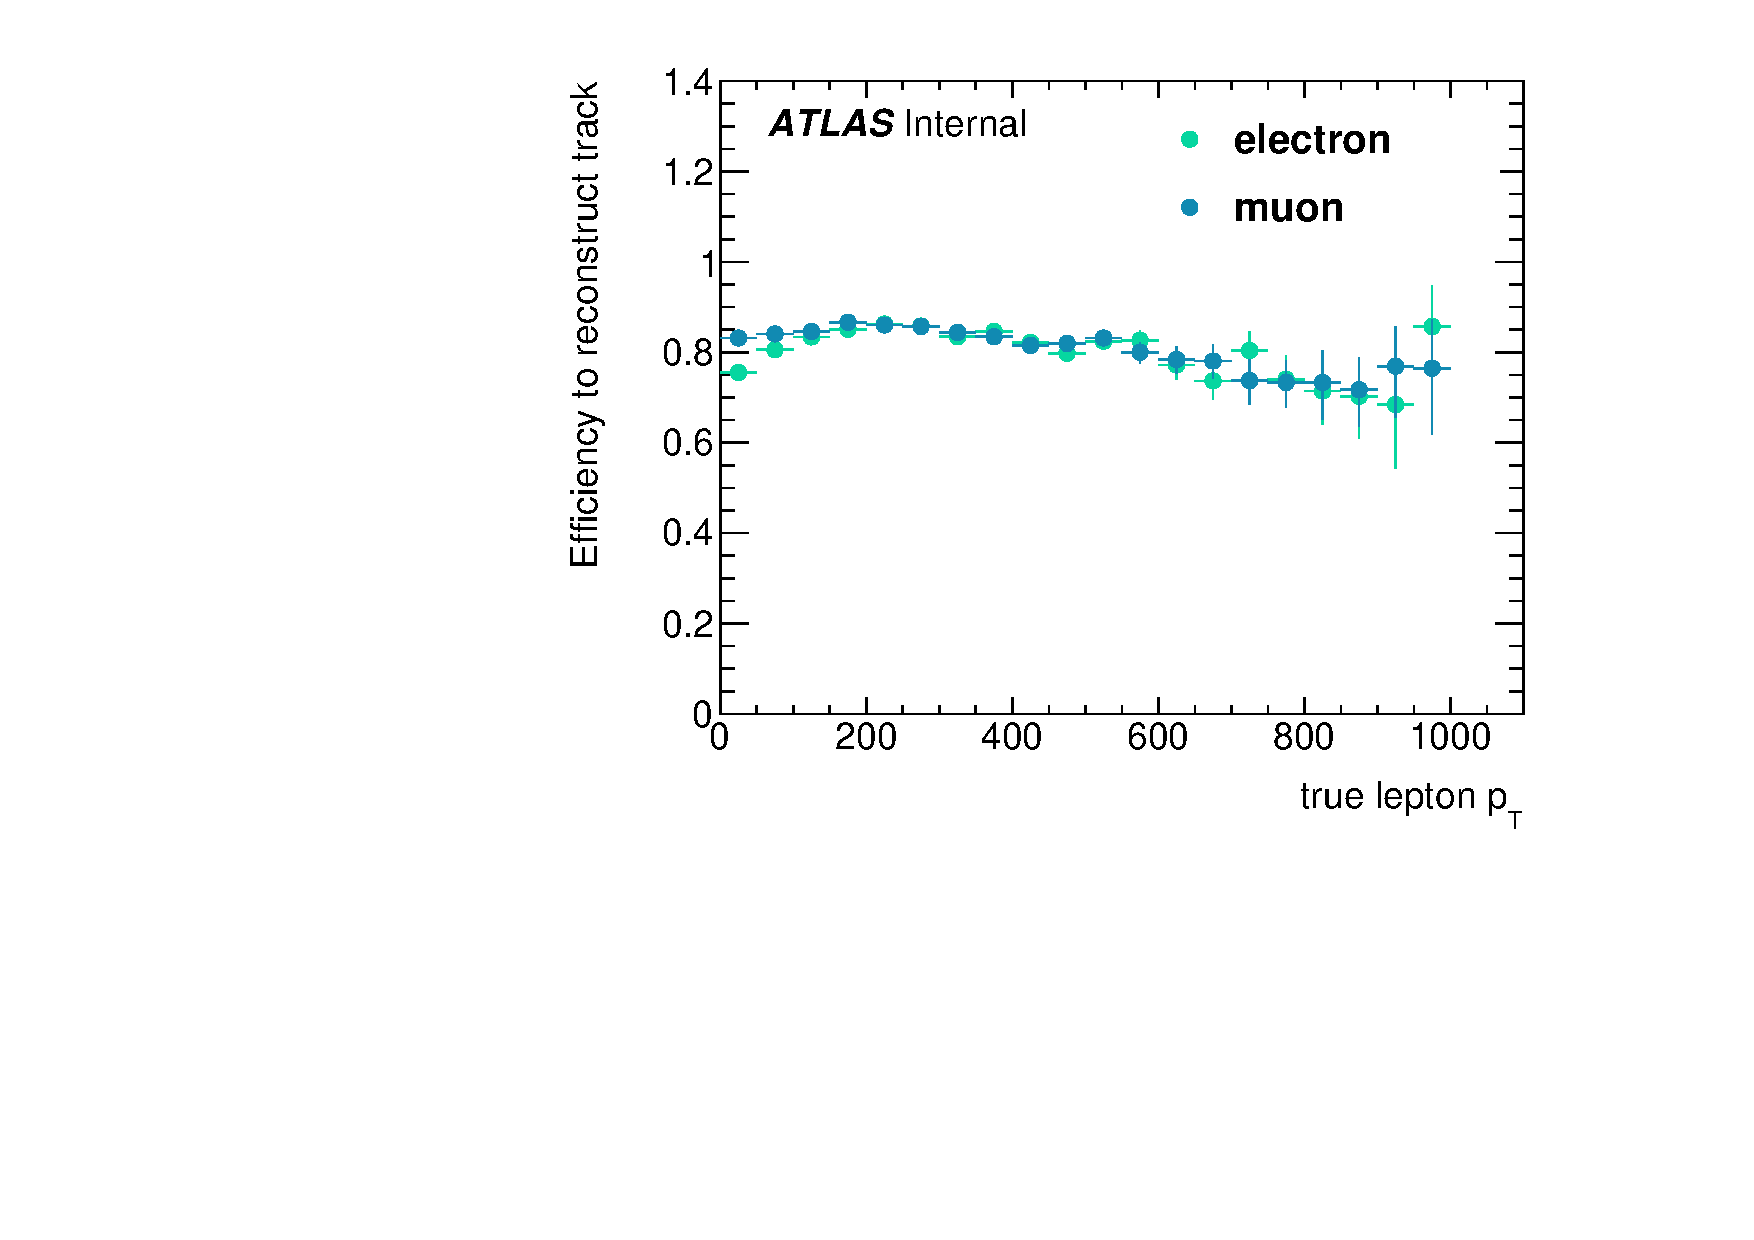
\includegraphics[width=.48\textwidth]{figures/LRT_systs/stlrt_compare_elmu_pt.pdf}
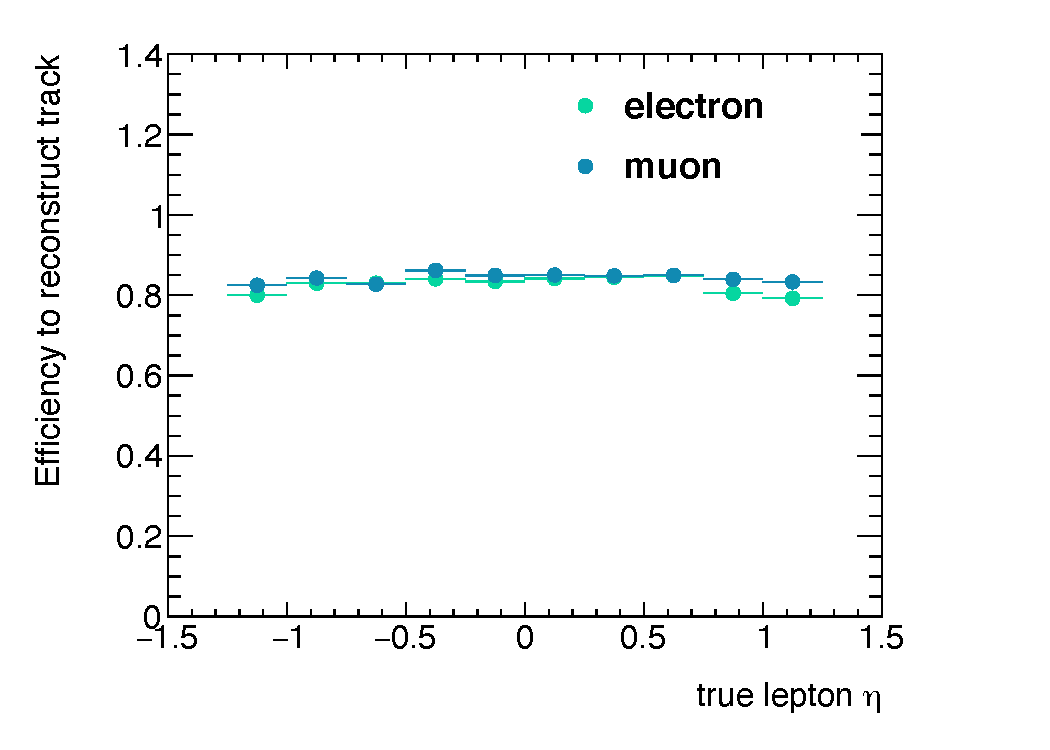
\includegraphics[width=.48\textwidth]{figures/LRT_systs/stlrt_compare_elmu_eta.pdf}
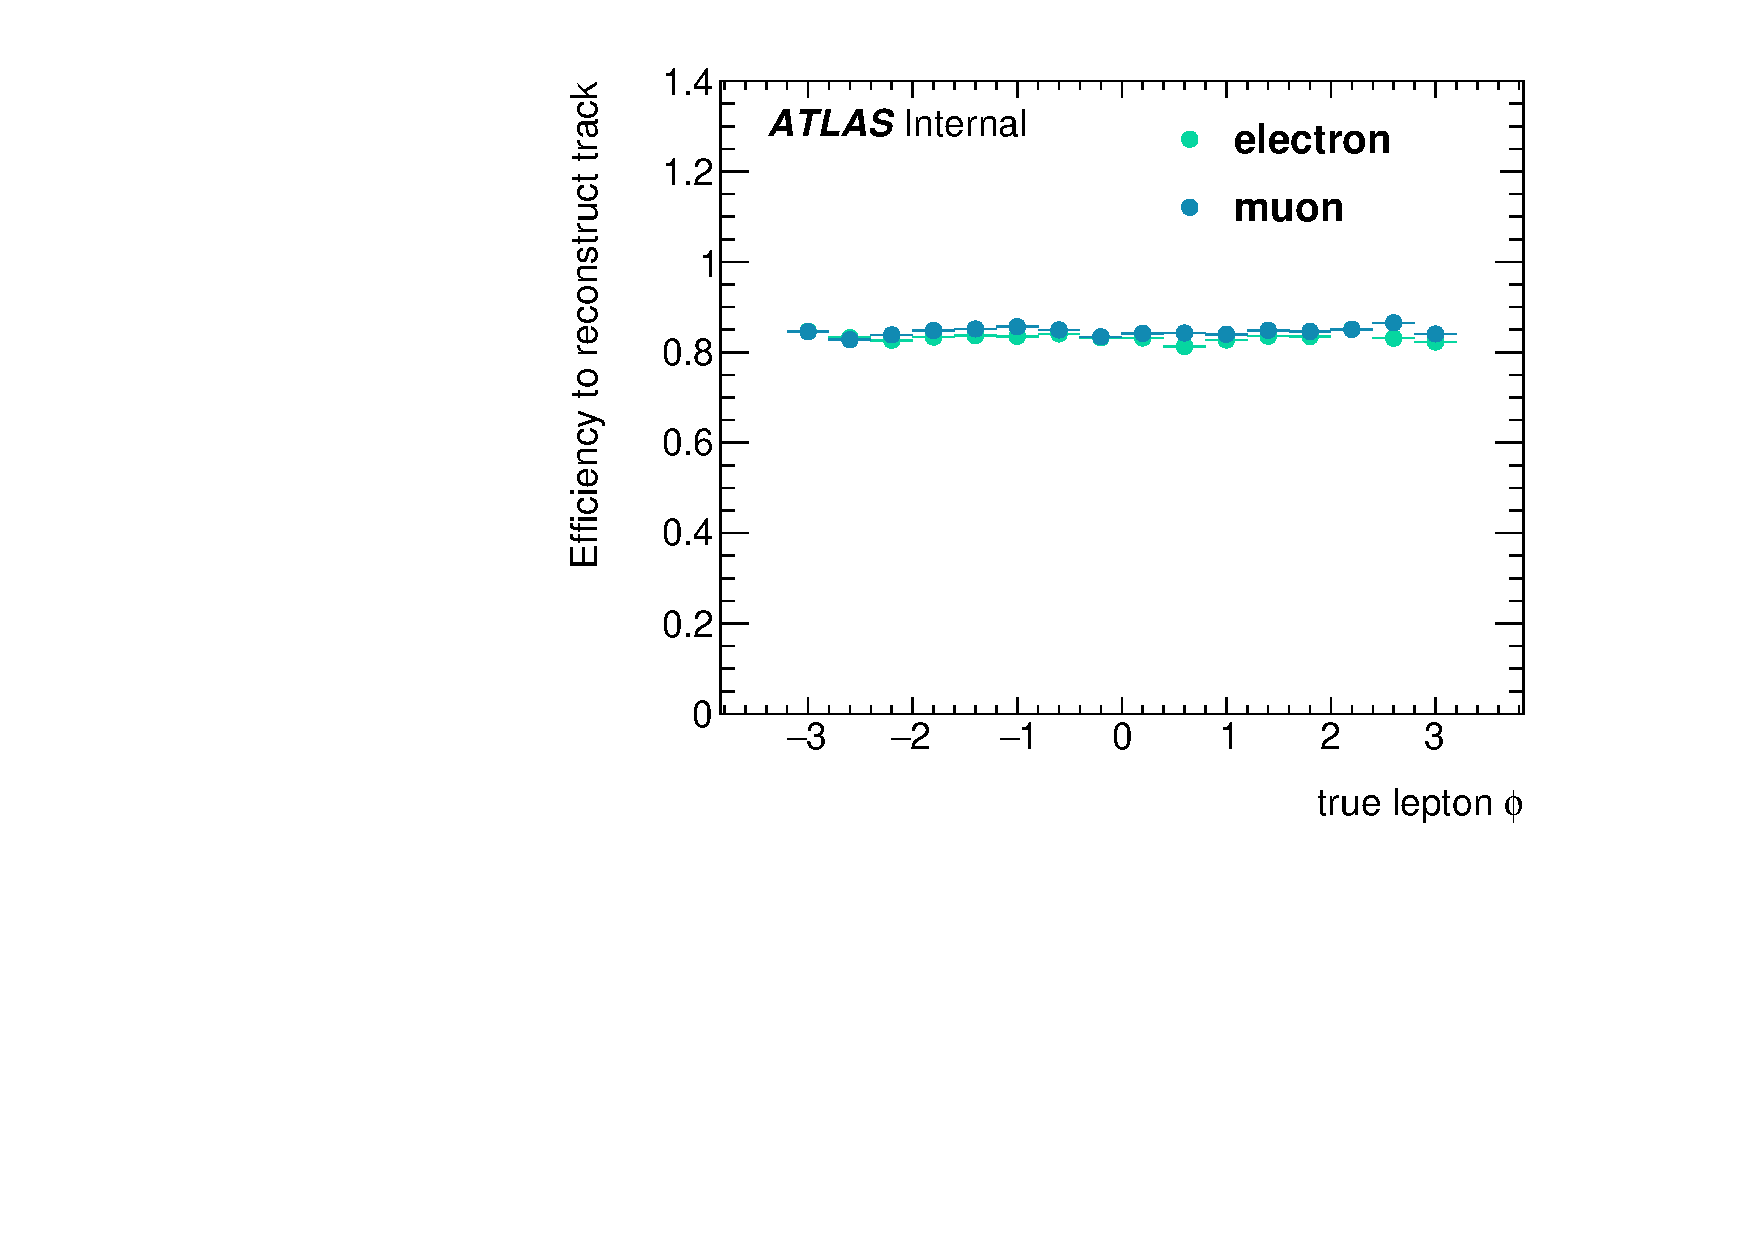
\includegraphics[width=.48\textwidth]{figures/LRT_systs/stlrt_compare_elmu_phi.pdf}
\caption{Tracking efficency for electrons and muons in signal MC (all lifetimes of 300 GeV \selec or \smu). These plots justify the assumpution that tracking efficiency is the same between electrons and muons and symmetric about the \ac{ID} volume.}
\label{fig:trk_el_mu}
\end{figure}

\begin{table}
\begin{tabular}{c}
Cut on cosmic muon \\
\hline
$\pt > 50 \GeV$ \\
$\absdz > 3$mm \\
$|\eta| < 1.05$ \\
$\absz < 120$ mm \\
$\tavg > 0$ if $\phi_{\mu} < 0$ OR $\tavg > 0$ if $\phi_{\mu} > 0$ \\
\hline
\end{tabular}
\quad
\begin{tabular}{c}
Cut on truth muon\\
\hline
$\pt > 50 \GeV$ \\
$\absdz > 3$mm \\
$|\eta| < 1.05$ \\
parent is a \smu \\
\dz and $R_{\textrm{decay}}$ between the same silicon layers\\
\hline
\end{tabular}
\caption{Cuts on tag muons. Cosmic muons (right) and truth signal muons (left).}
\label{tab:lrt-mu-cuts}
\end{table}

\begin{table}
\centering
\begin{tabular}{c}
Cut on cosmic muon \\
\hline
$\pt > 30 \GeV$ \\
$\Delta R_{\textrm{cos}}= \sqrt{ (\Delta \phi - \pi)^{2} + (\Sigma \eta)^{2}} < 0.3$ \\
$|d_{0, \textrm{track}} - d_{0, \mu}| < 20$ \\
$|z_{0, \textrm{track}} - z_{0, \mu}| < 20$ \\
\hline
\end{tabular}
\quad
\quad
\begin{tabular}{c}
Cut on truth muon\\
\hline
$\pt > 30 \GeV$ \\
$\Delta R = \sqrt{ (\Delta \phi)^{2} + (\Delta \eta)^{2}} < 0.05$ \\
 \\
 \\
\hline
\end{tabular}
\caption{Cuts on probe \ac{ID} tracks. In data (right) and signal (left).}
\label{tab:lrt-track-cuts}
\end{table}



\begin{figure}[htbp]
\centering
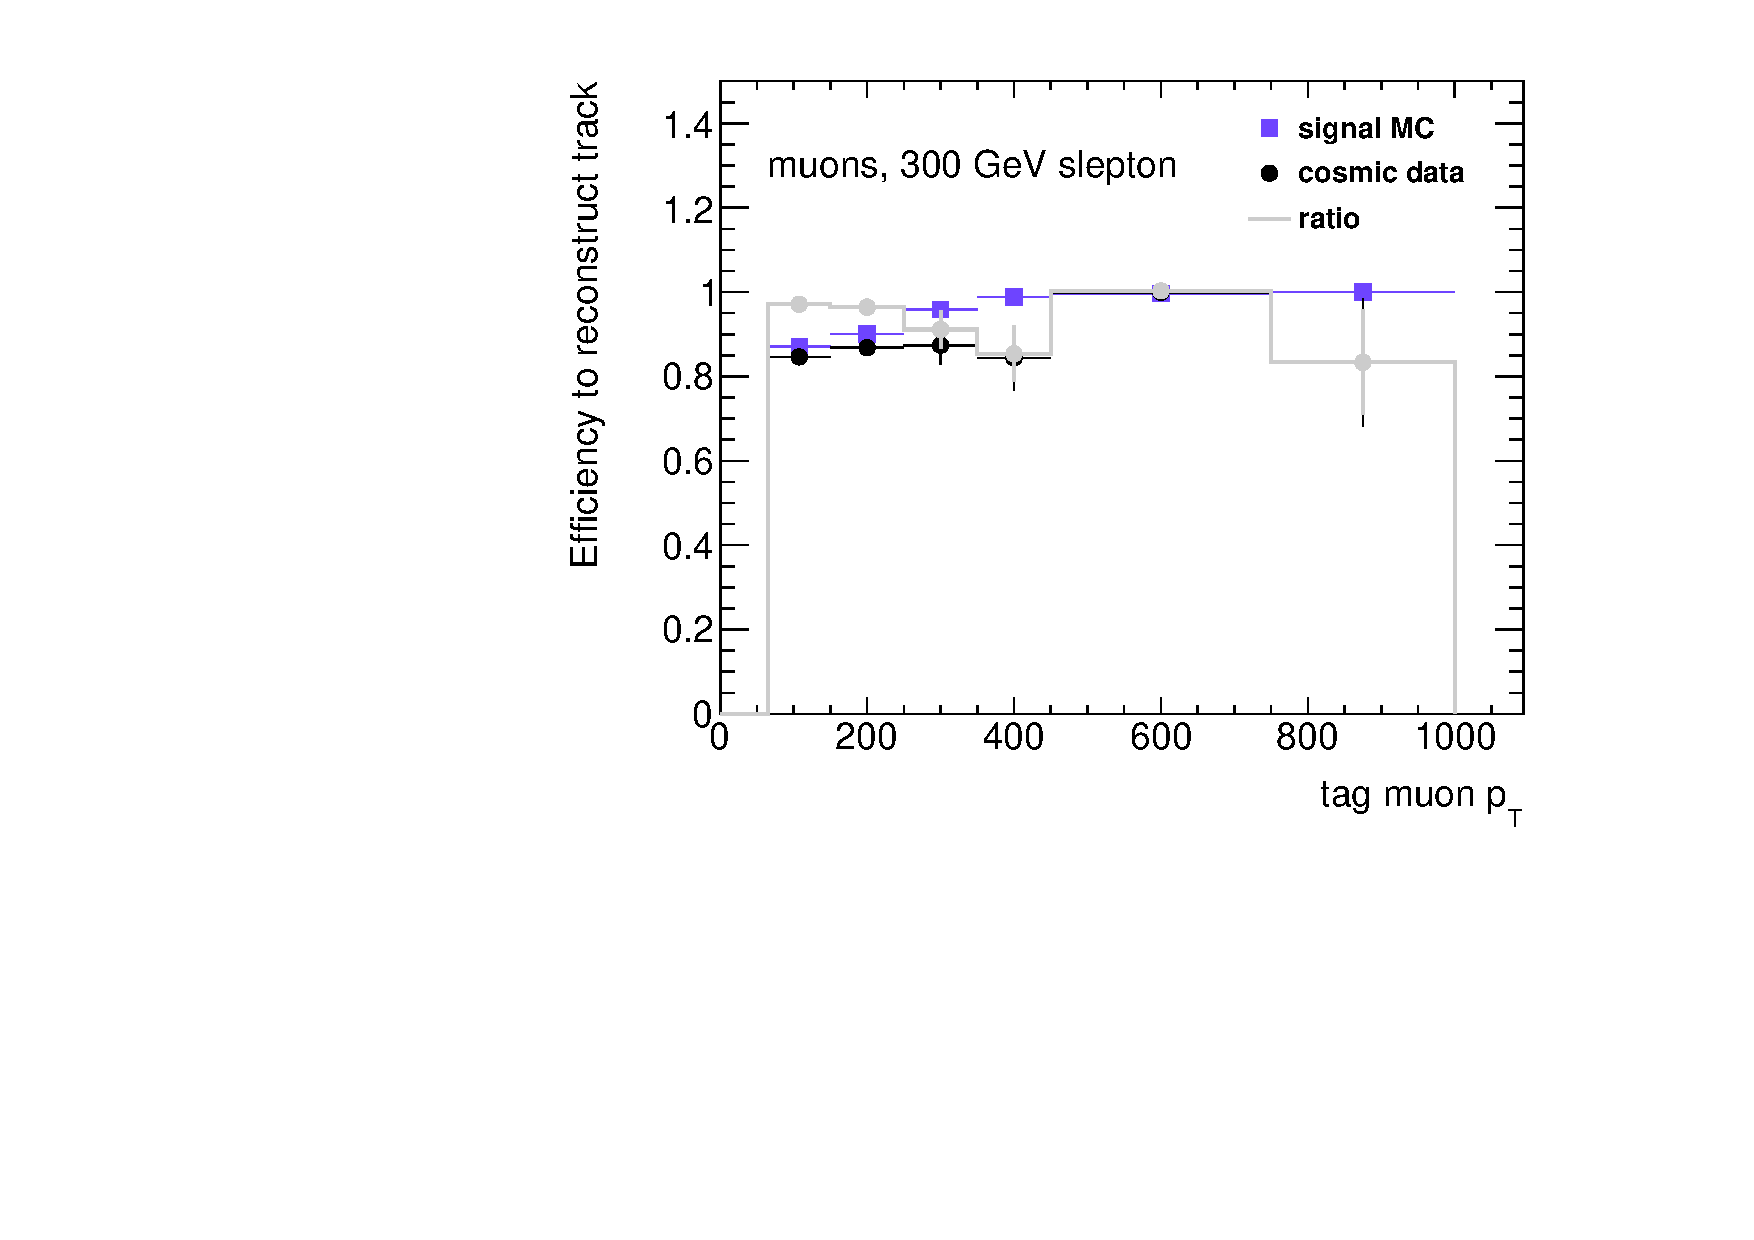
\includegraphics[width=.48\textwidth]{figures/LRT_systs/compare_pt_z0120_Rgd0_timing_idcuts_2dweight.pdf}
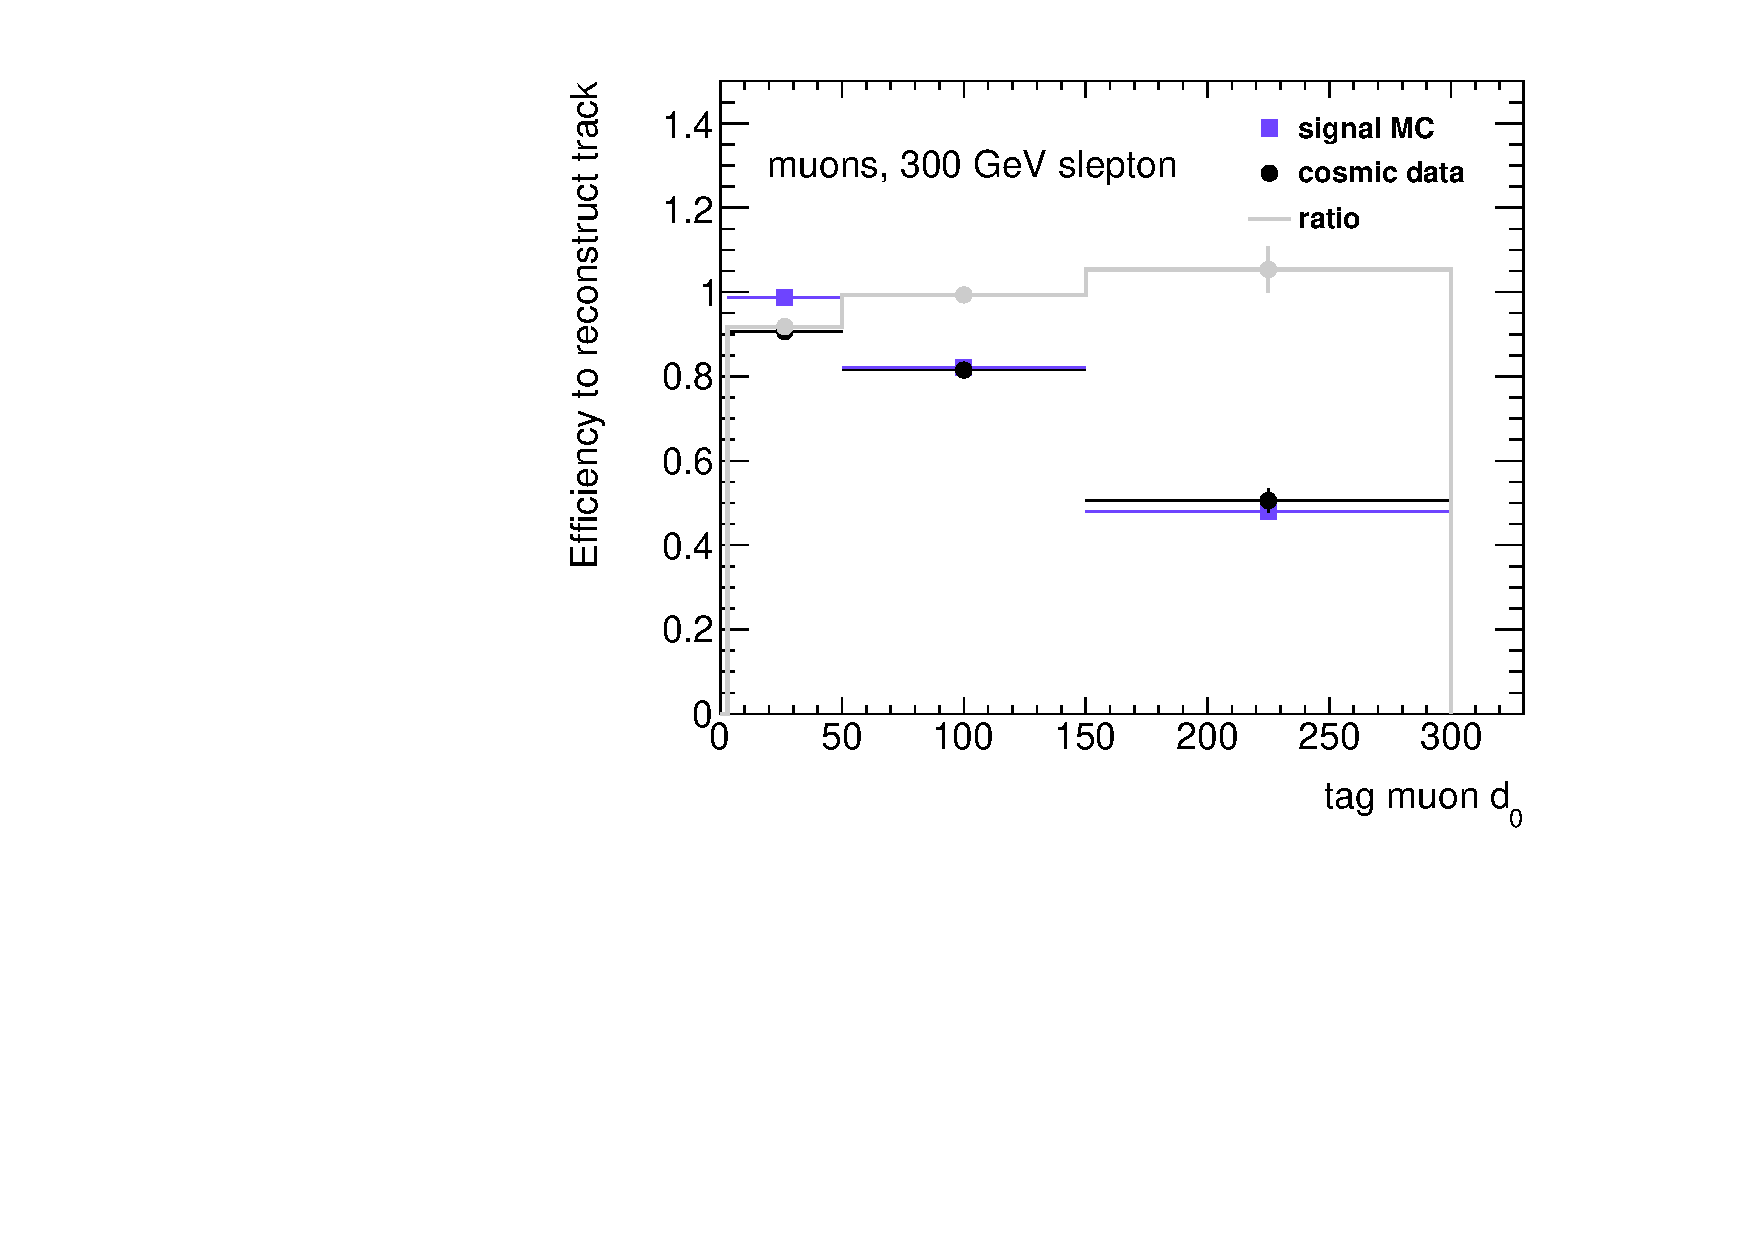
\includegraphics[width=.48\textwidth]{figures/LRT_systs/compare_d0_z0120_Rgd0_timing_idcuts_2dweight.pdf}
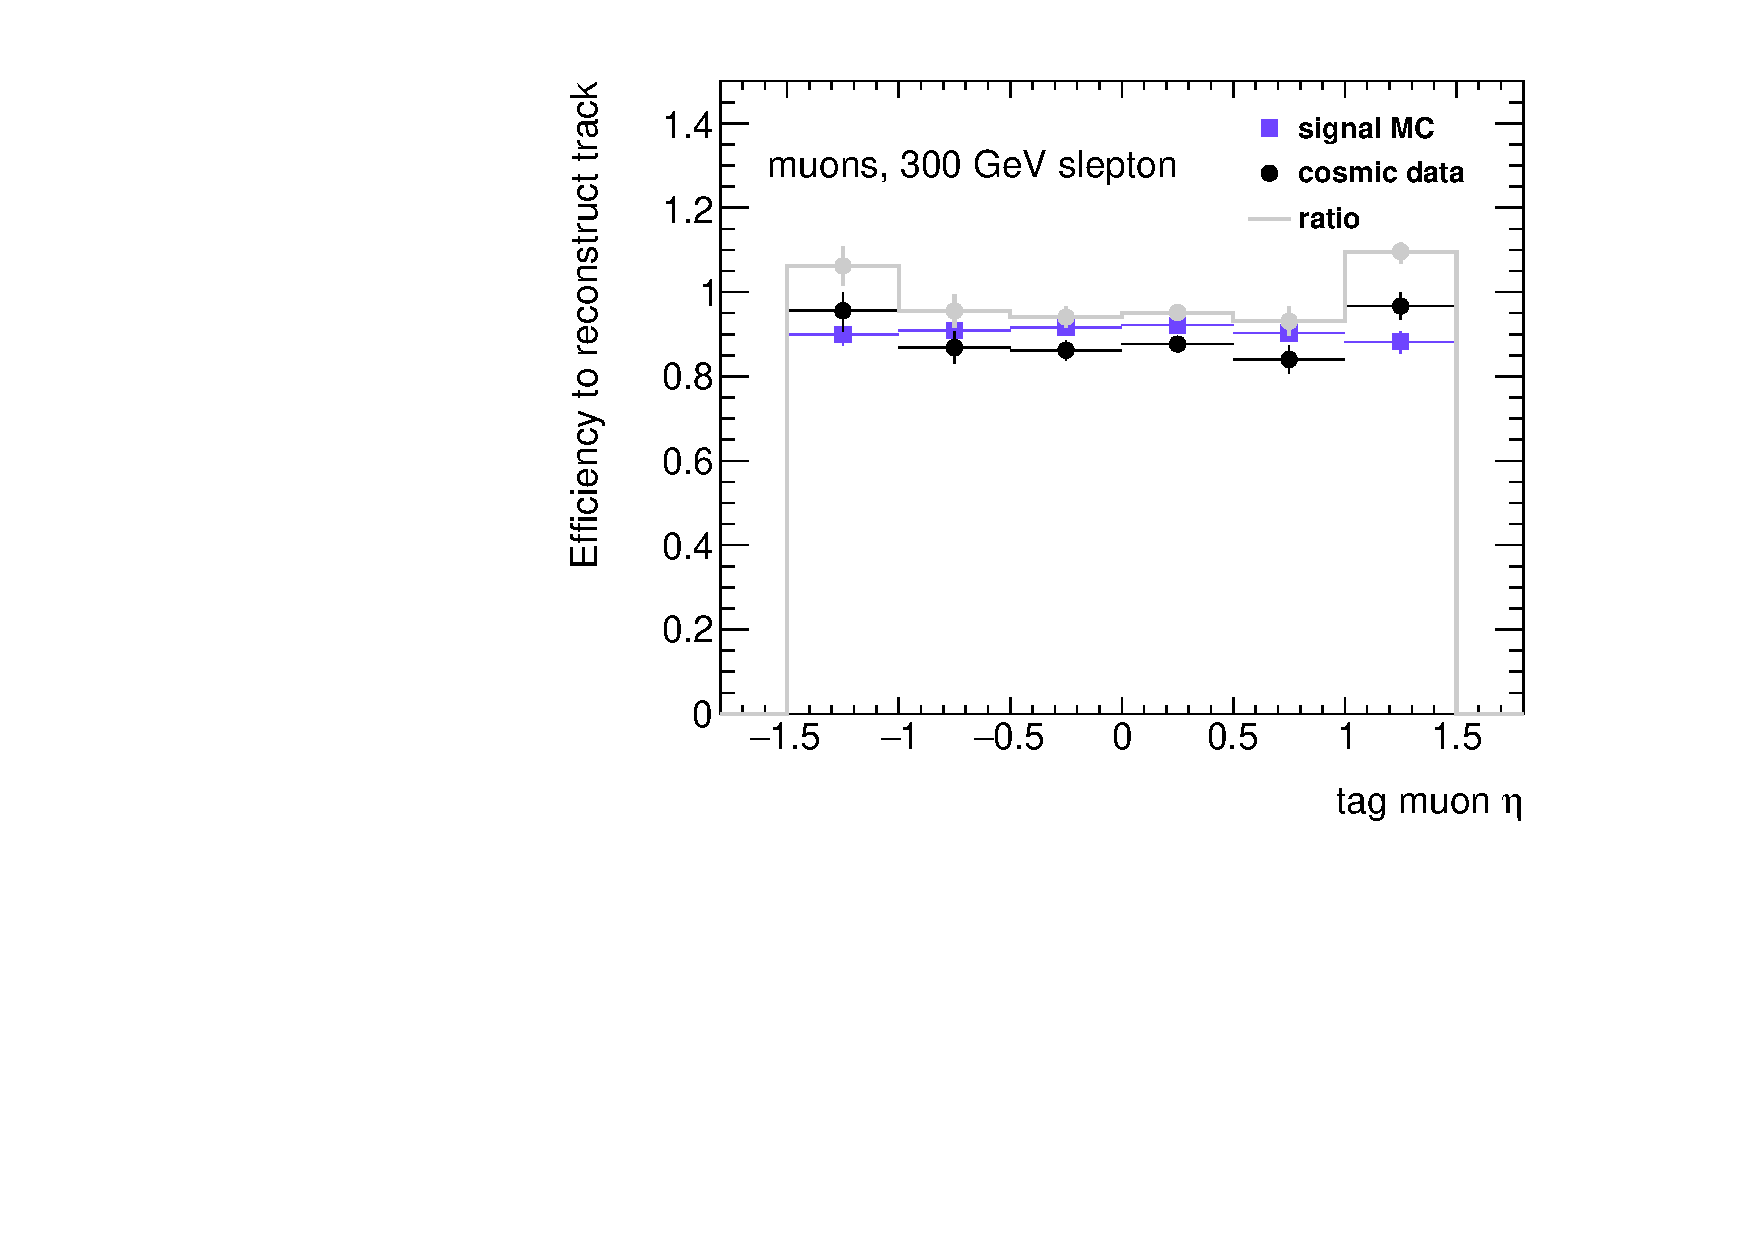
\includegraphics[width=.48\textwidth]{figures/LRT_systs/compare_eta_z0120_Rgd0_timing_idcuts_2dweight.pdf}
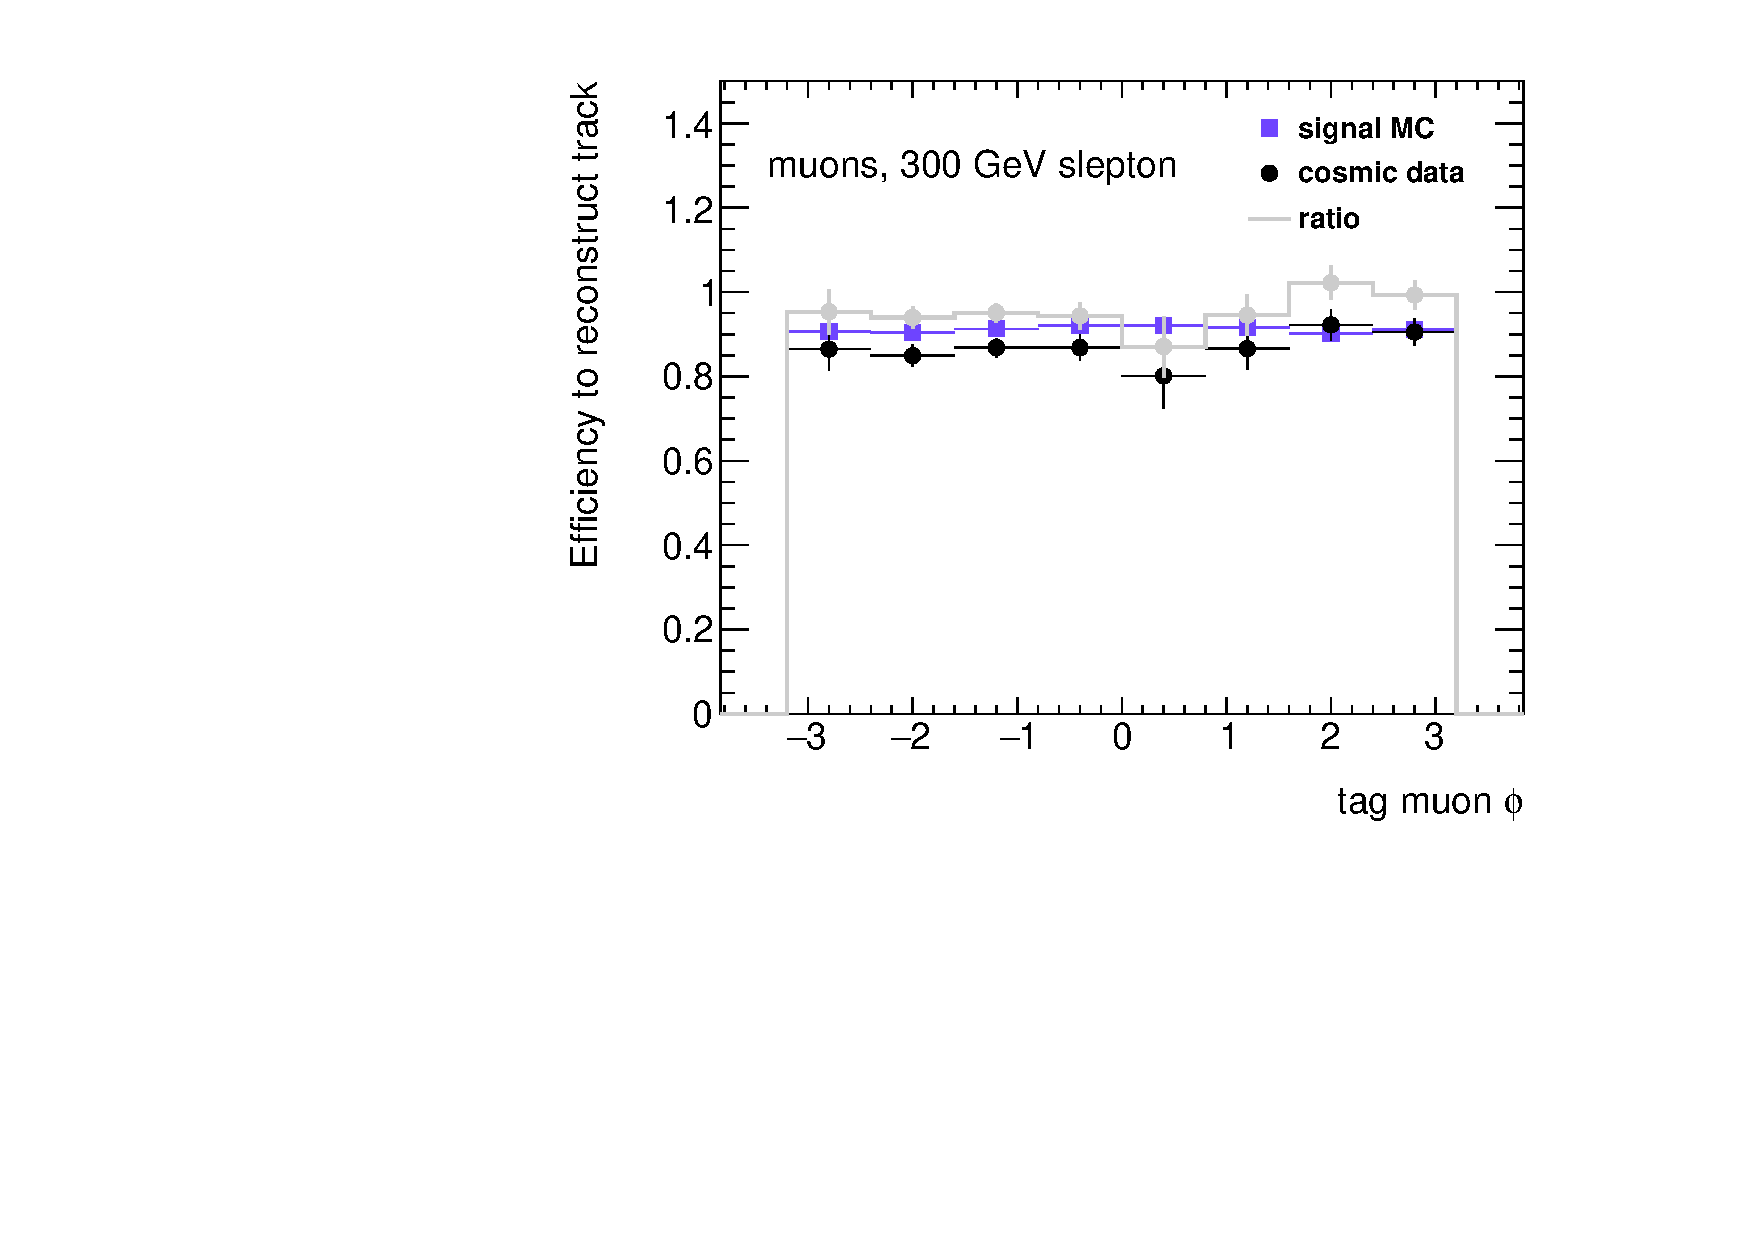
\includegraphics[width=.48\textwidth]{figures/LRT_systs/compare_phi_z0120_Rgd0_timing_idcuts_2dweight.pdf}
\caption{A comparison of tracking efficiency in cosmics data and signal MC (all masses and lifetimes can be used to due the eventual \pt and \dz binning) with respect to \pt (top left), \dz (top right), $\eta$ (bottom left), and $\phi$ (bottom right). The \ac{MC} efficiency is shown in purple, the data efficiency in black, and the ratio between the efficienceis is shown in gray.}
\label{fig:lrt_eff_comp}
\end{figure}




\subsection{Lepton Displacement}

The effect of displacement on lepton reconstruction cannot be directly compared between data and \ac{MC}. An additional uncertainty is defined in \ac{MC} to account for reconstruction effects potentially not captured by the previous two systematic uncertainties. It is taken as the deviation in the reconstruction efficiency as a function of \absdz relative to prompt muons.
This uncertainty is meant to capture any discrepancy in \ac{MS} track or electron shower shape parameters at high \absdz, as well as changes in how they are combined with the \ac{ID} track. This uncertainty is extremely conservative as there is no way to determine if the same fluctations are seen in data.


To determine the systematic uncertainty due to displaced reconstruction, the baseline or signal reconstruction/selection efficiency is divided by the tracking efficiency in order to separate any inefficiences from \ac{LRT}. Then, the ratio of each high \dz bin relative the prompt bin (0--3 mm) is taken, results of this are shown in Fig.~\ref{fig:disp_systs}. The uncertainty is assigned to each lepton and they are summed in quadrature to get an event level systematic. 


This uncertainty for muons is quite small, while it is much more substantial for electrons. Electrons are identified using a likelihood, which is trained with \dz as a discriminating variable. \absdz was removed from the cuts performed offline, but the LH was not retrained, and so there as a larger relic \dz dependence and the displacement uncertainty is much larger.


\begin{figure}[htbp]
\centering
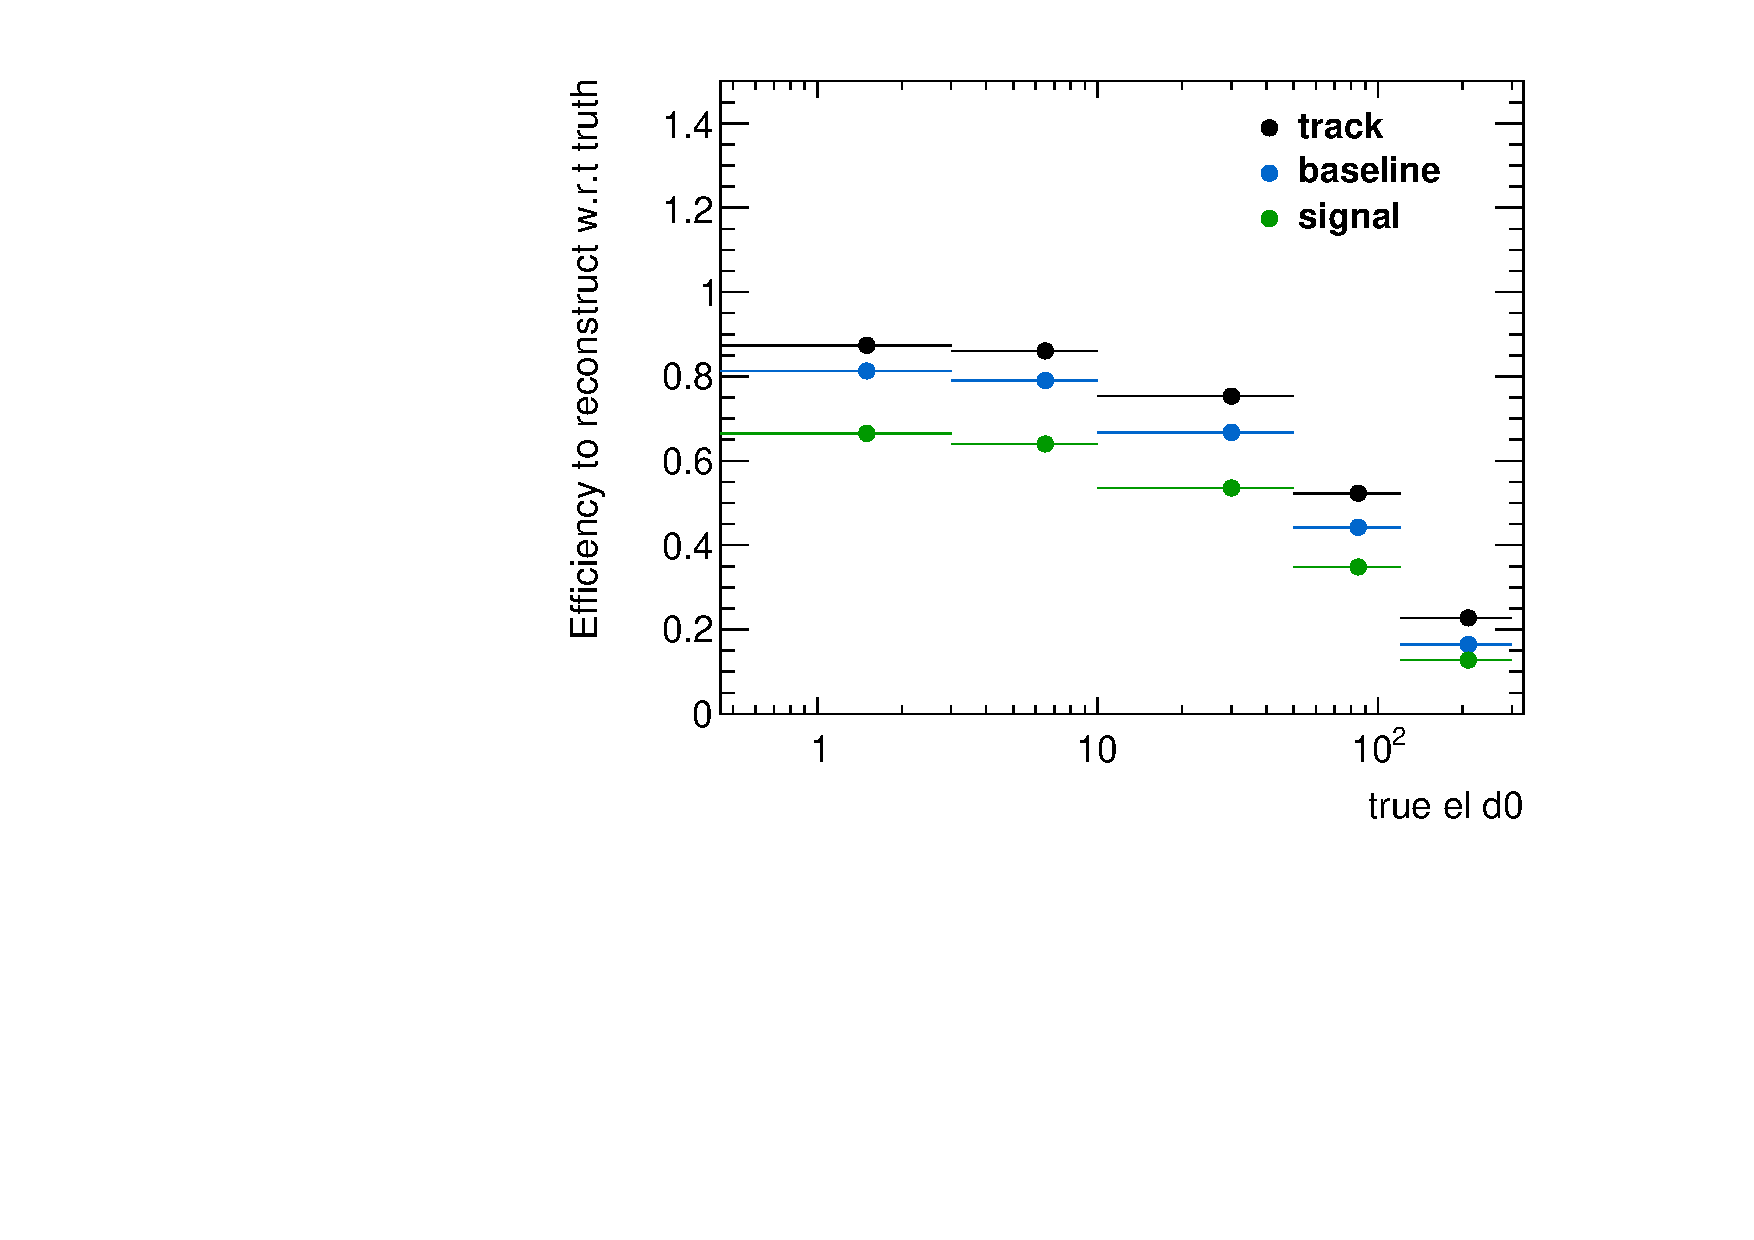
\includegraphics[width=.48\textwidth]{figures/disp_systs/signal_effcompare_d0_el_300.pdf}
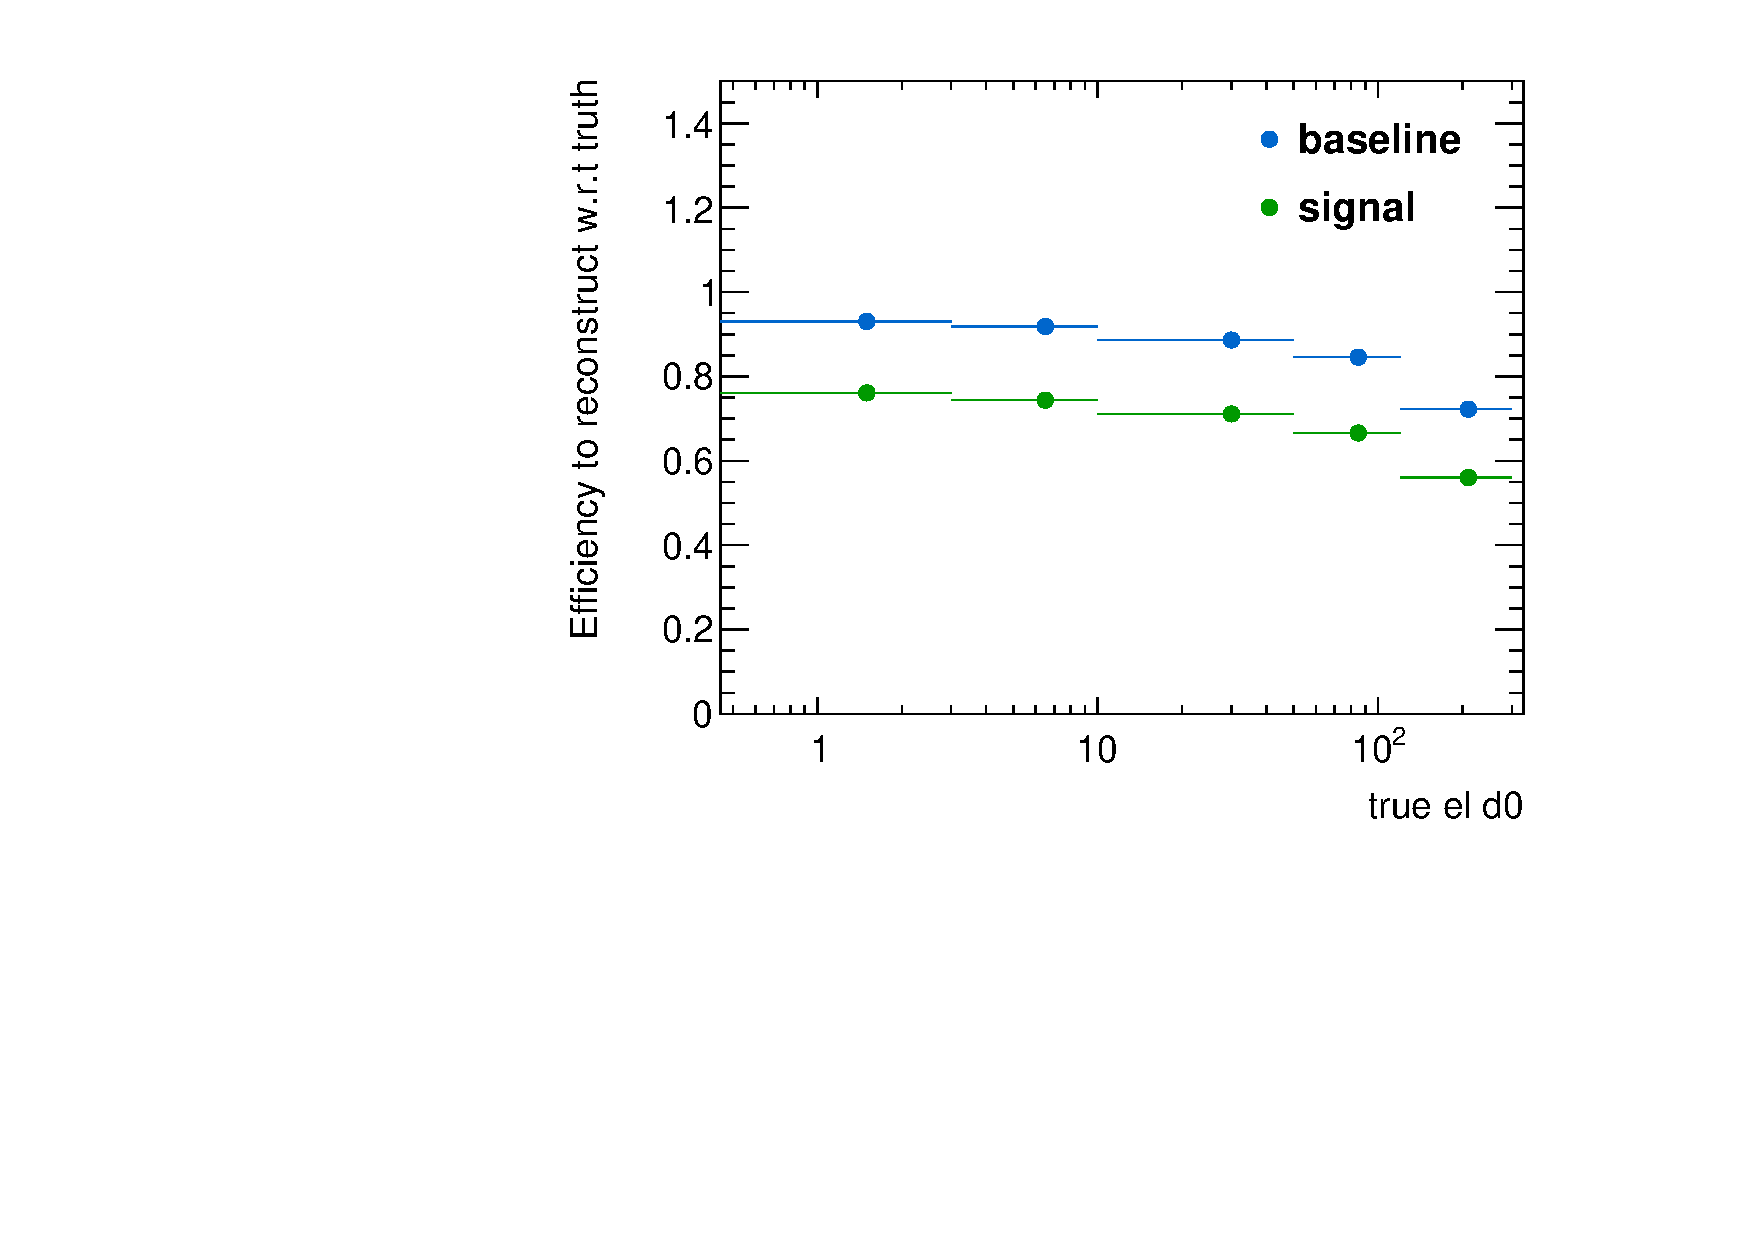
\includegraphics[width=.48\textwidth]{figures/disp_systs/signal_effwrttrack_d0_el_300.pdf}
\caption{Electron selection efficiencies with respect to truth (left) and with respect to the tracking efficiency (right). Made from a 300 GeV \slep signal samples with lifetimes between 0.01 ns-1 ns. The denominator of the efficiency is truth electrons from \selec with $\pt > 65 \GeV$ and $|\eta| < 2.5$, and the numerator is truth matched and signal (or baseline) quality tracks or leptons.}
\label{fig:disp_el}
\end{figure}

\begin{figure}[htbp]
\centering
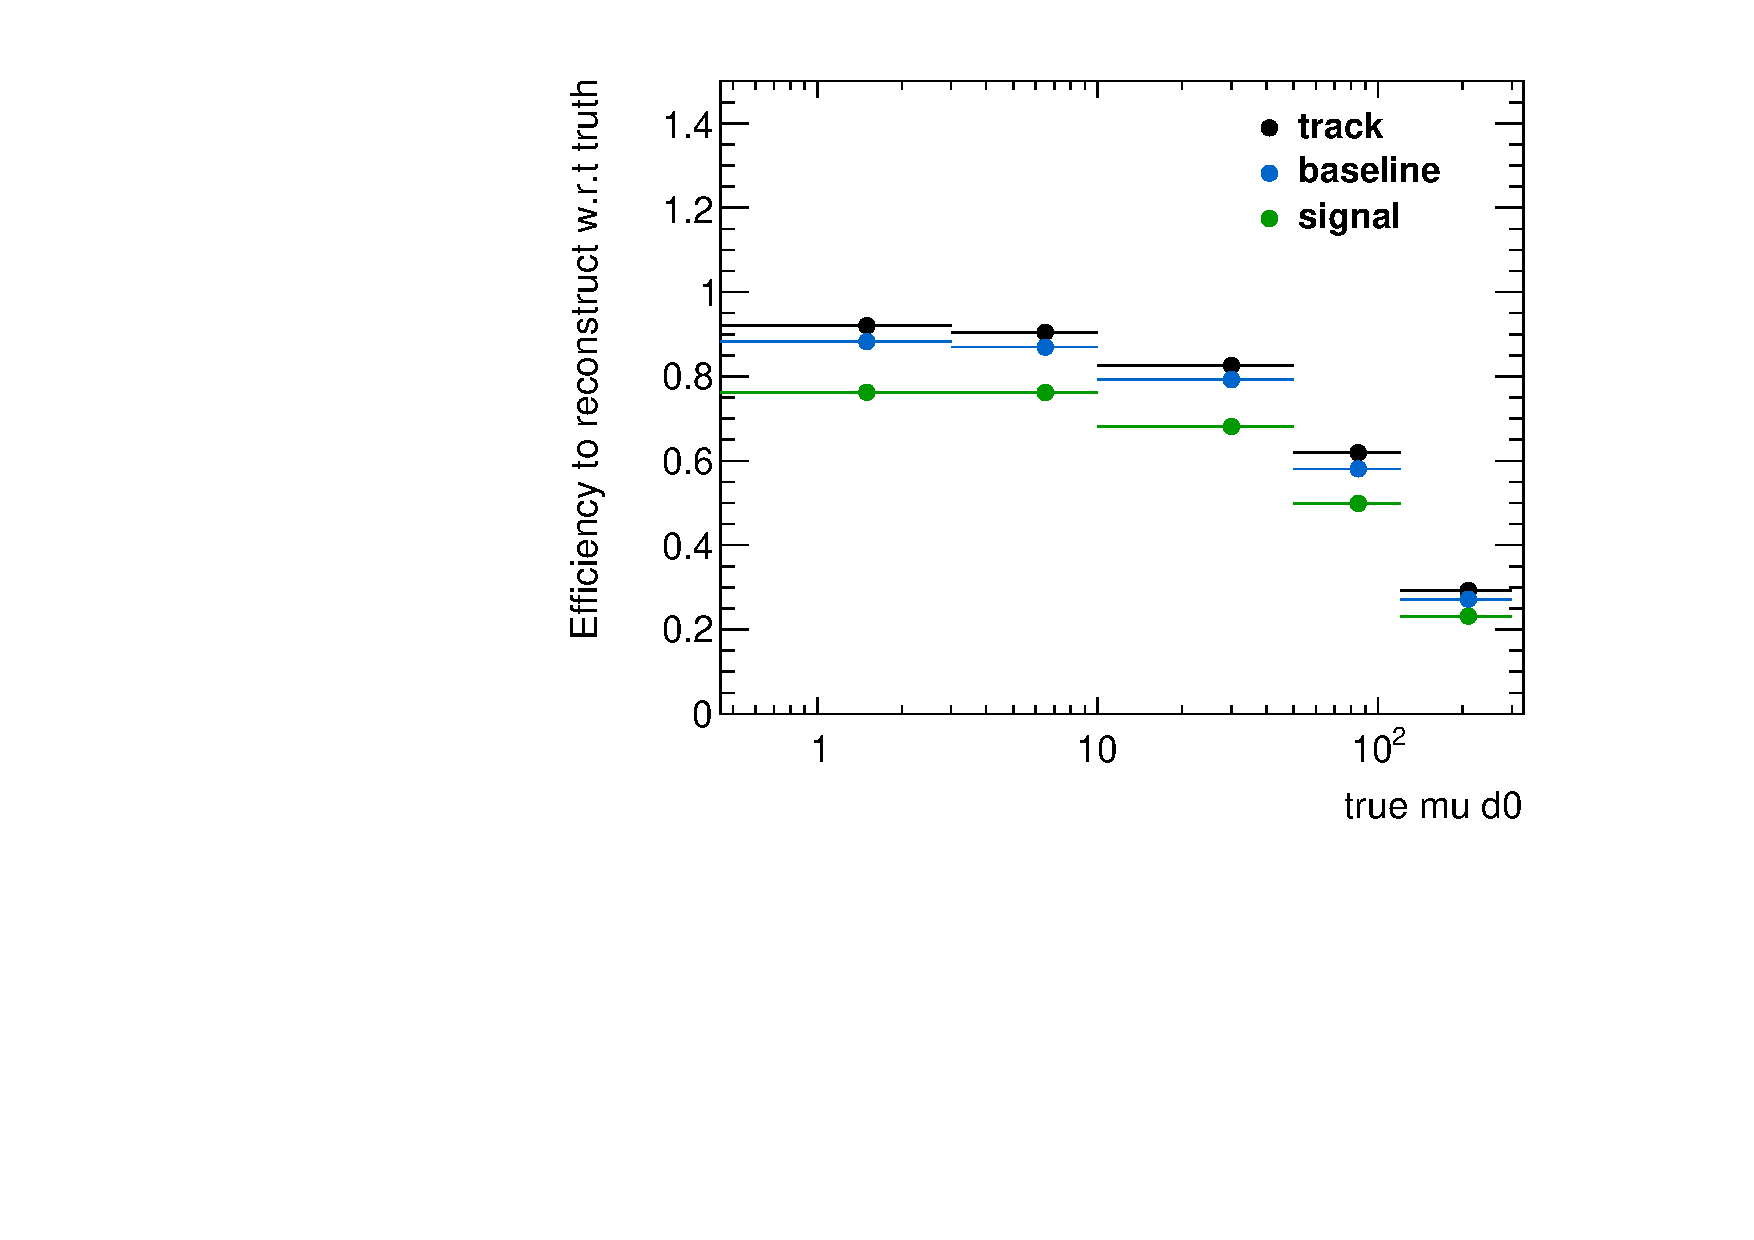
\includegraphics[width=.48\textwidth]{figures/disp_systs/signal_effcompare_d0_mu_300.pdf}
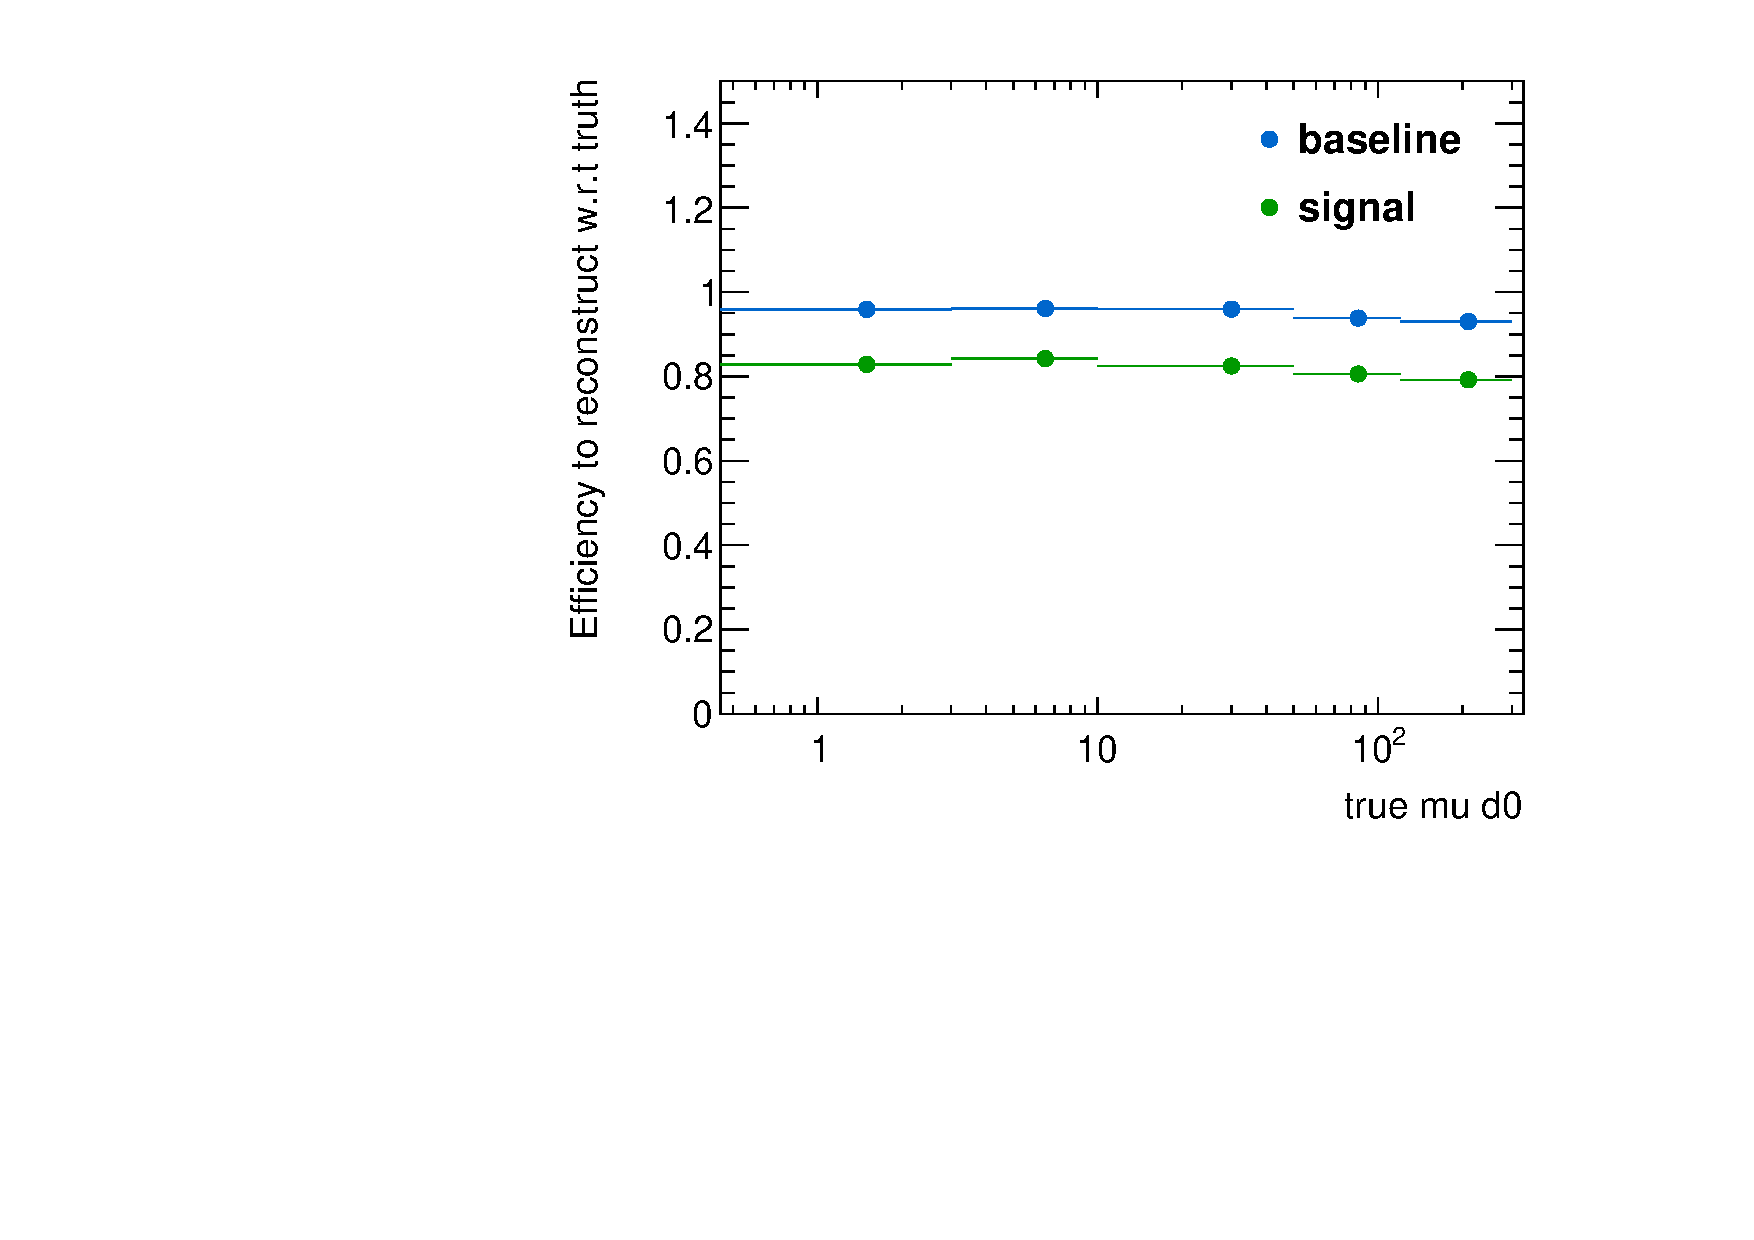
\includegraphics[width=.48\textwidth]{figures/disp_systs/signal_effwrttrack_d0_mu_300.pdf}
\caption{Muon selection efficiencies with respect to truth (left) and with respect to the tracking efficiency (right). Made from 300 GeV \slep signal samples with lifetimes between 0.0 1ns-1 ns. The denominator of the efficiency is truth muons from \smu with $\pt > 65 \GeV$ and $|\eta| < 2.5$, and the numerator is truth matched and signal (or baseline) quality tracks or leptons.}
\label{fig:disp_mu}
\end{figure}

\begin{figure}[htbp]
\centering
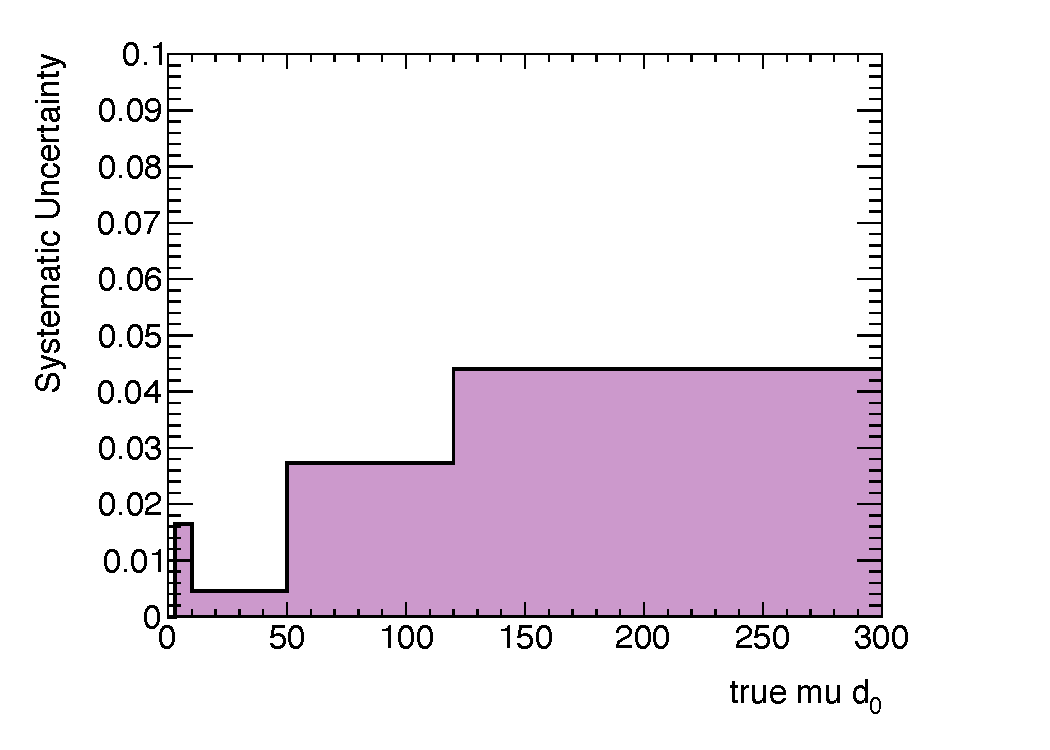
\includegraphics[width=.48\textwidth]{figures/disp_systs/signal_sf_d0_mu_300.pdf}
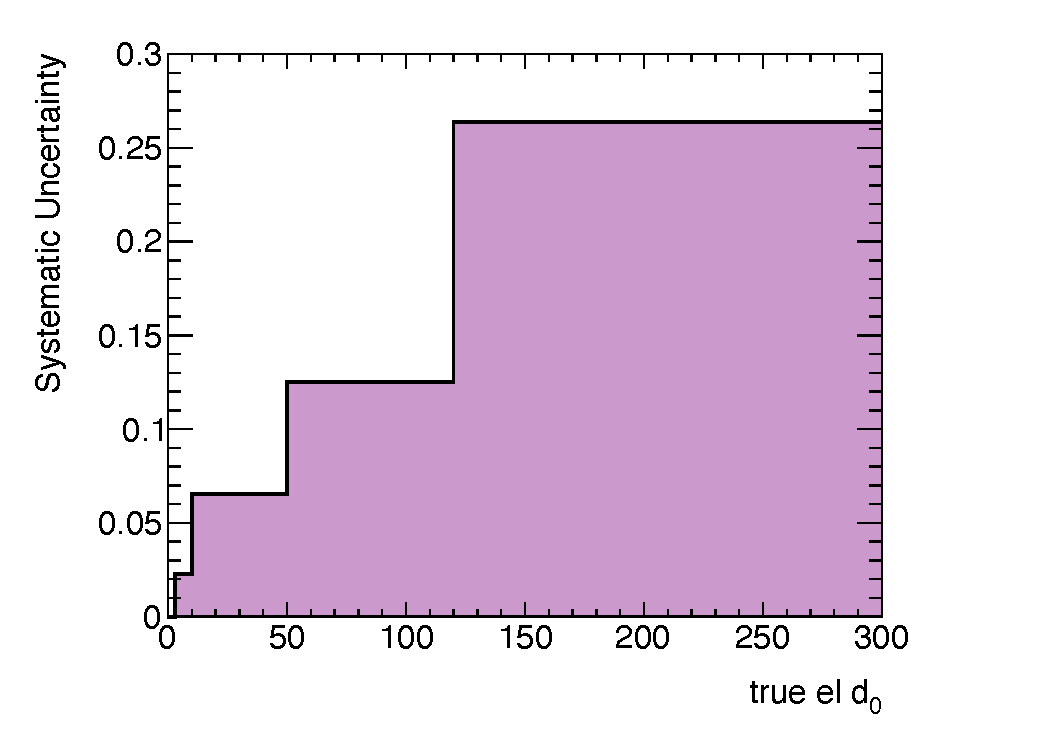
\includegraphics[width=.48\textwidth]{figures/disp_systs/signal_sf_d0_el_300.pdf}
\caption{Fractional systematic uncertainties defined for muons (left) and electrons. The value of each bin is defined as 1 minus the ratio of the selection efficiency with respect to tracking efficiency of the given bin to the same value of the prompt (0-3 mm) bin. These are defined in 300 GeV \slep signal samples with lifetimes between 0.01 ns-1 ns. It was confirmed that the trends are consistent across various \slep masses.}
\label{fig:disp_systs}
\end{figure}


%\begin{figure}[htbp]
%\centering
%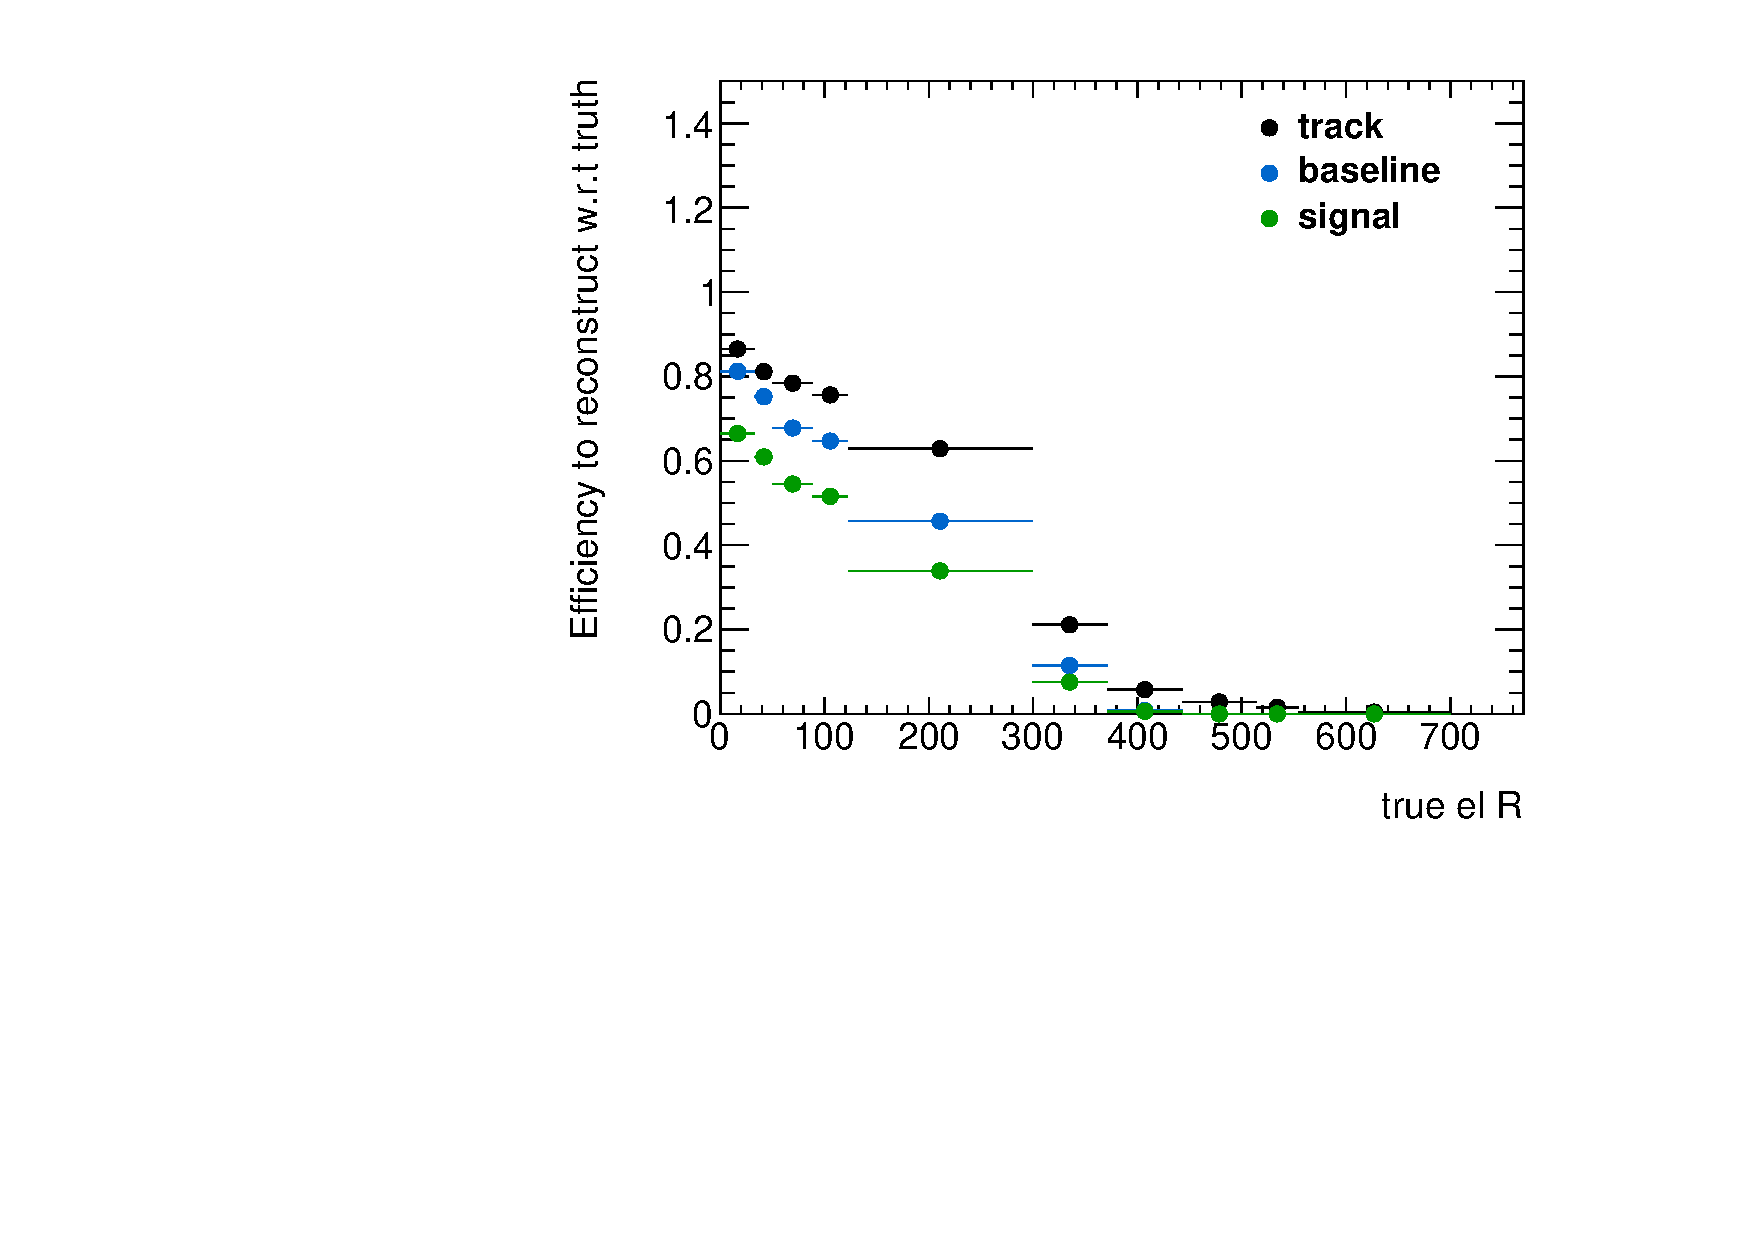
\includegraphics[width=.48\textwidth]{figures/disp_systs/signal_effcompare_R_el_300.pdf}
%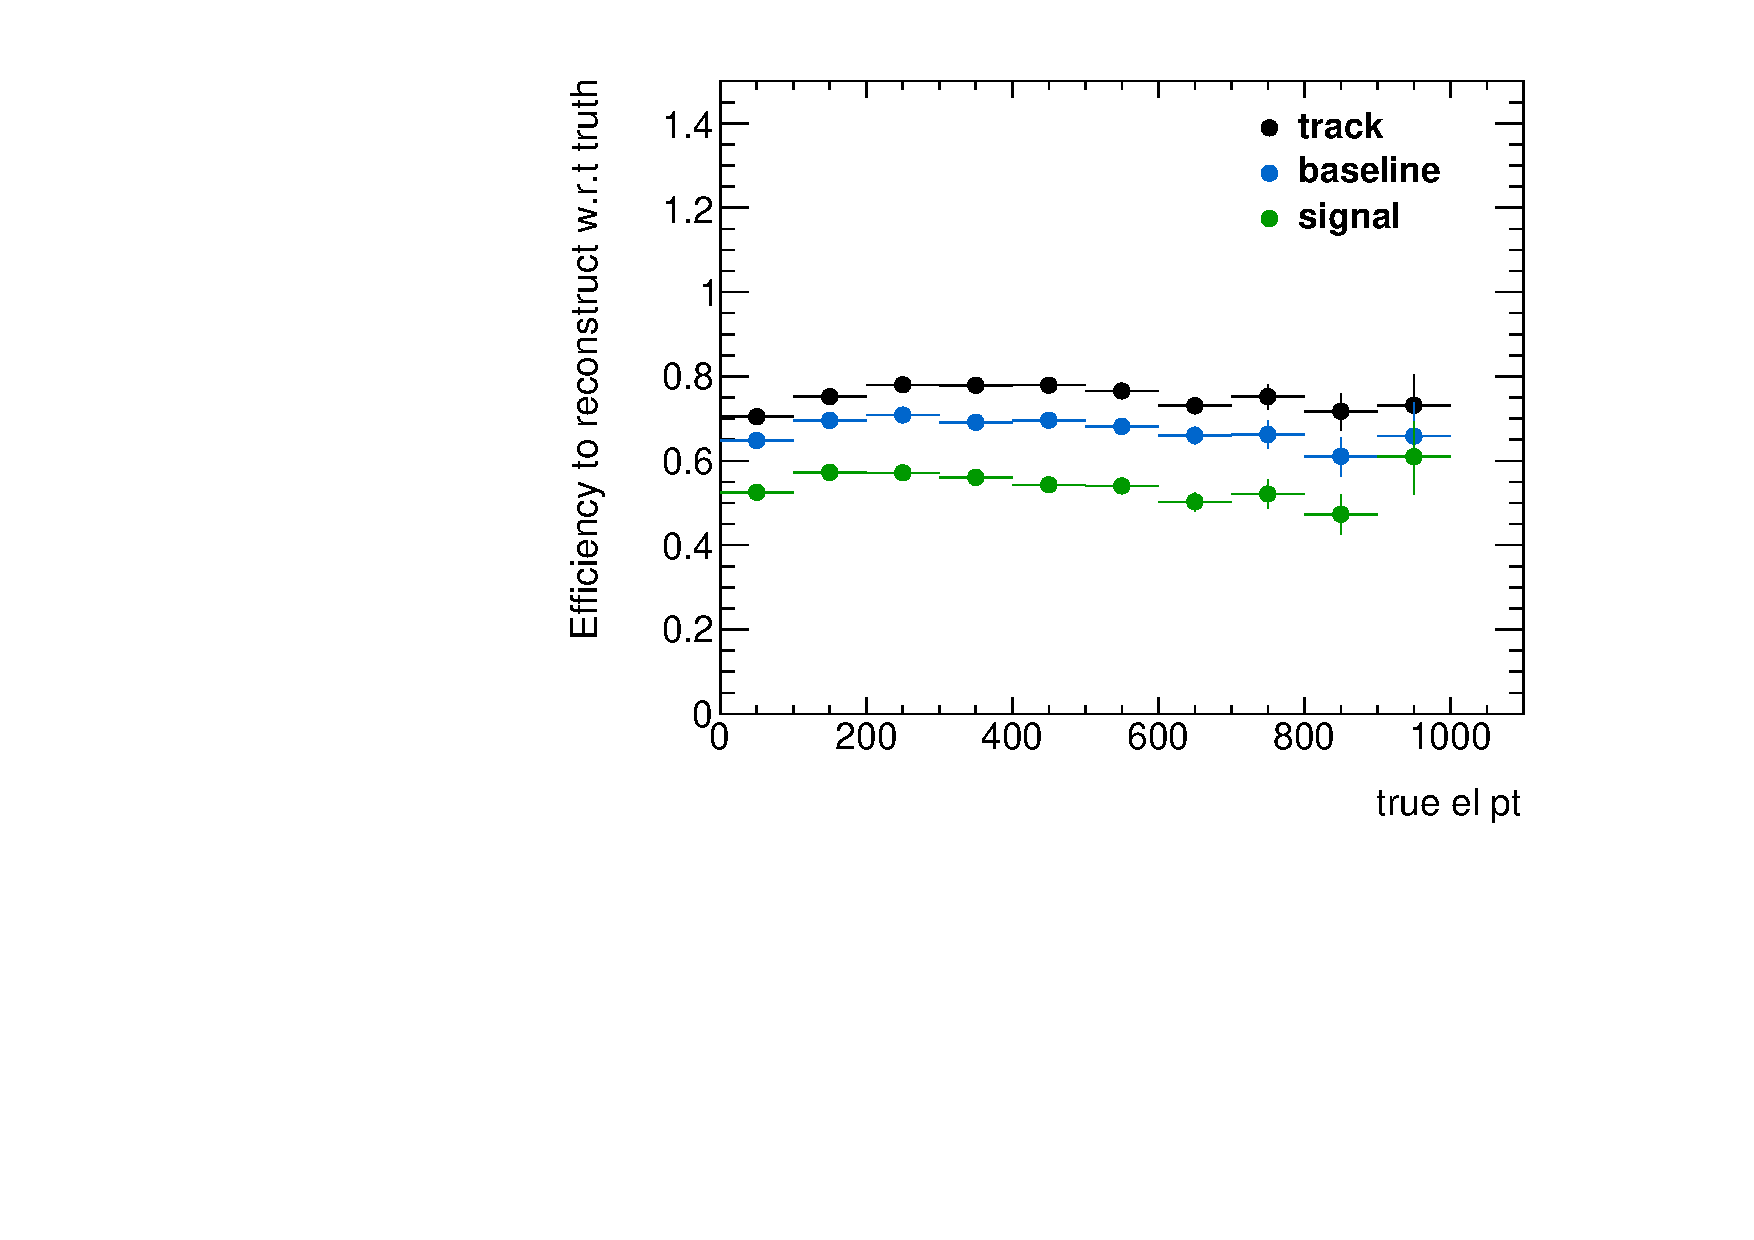
\includegraphics[width=.48\textwidth]{figures/disp_systs/signal_effcompare_pt_el_300.pdf}
%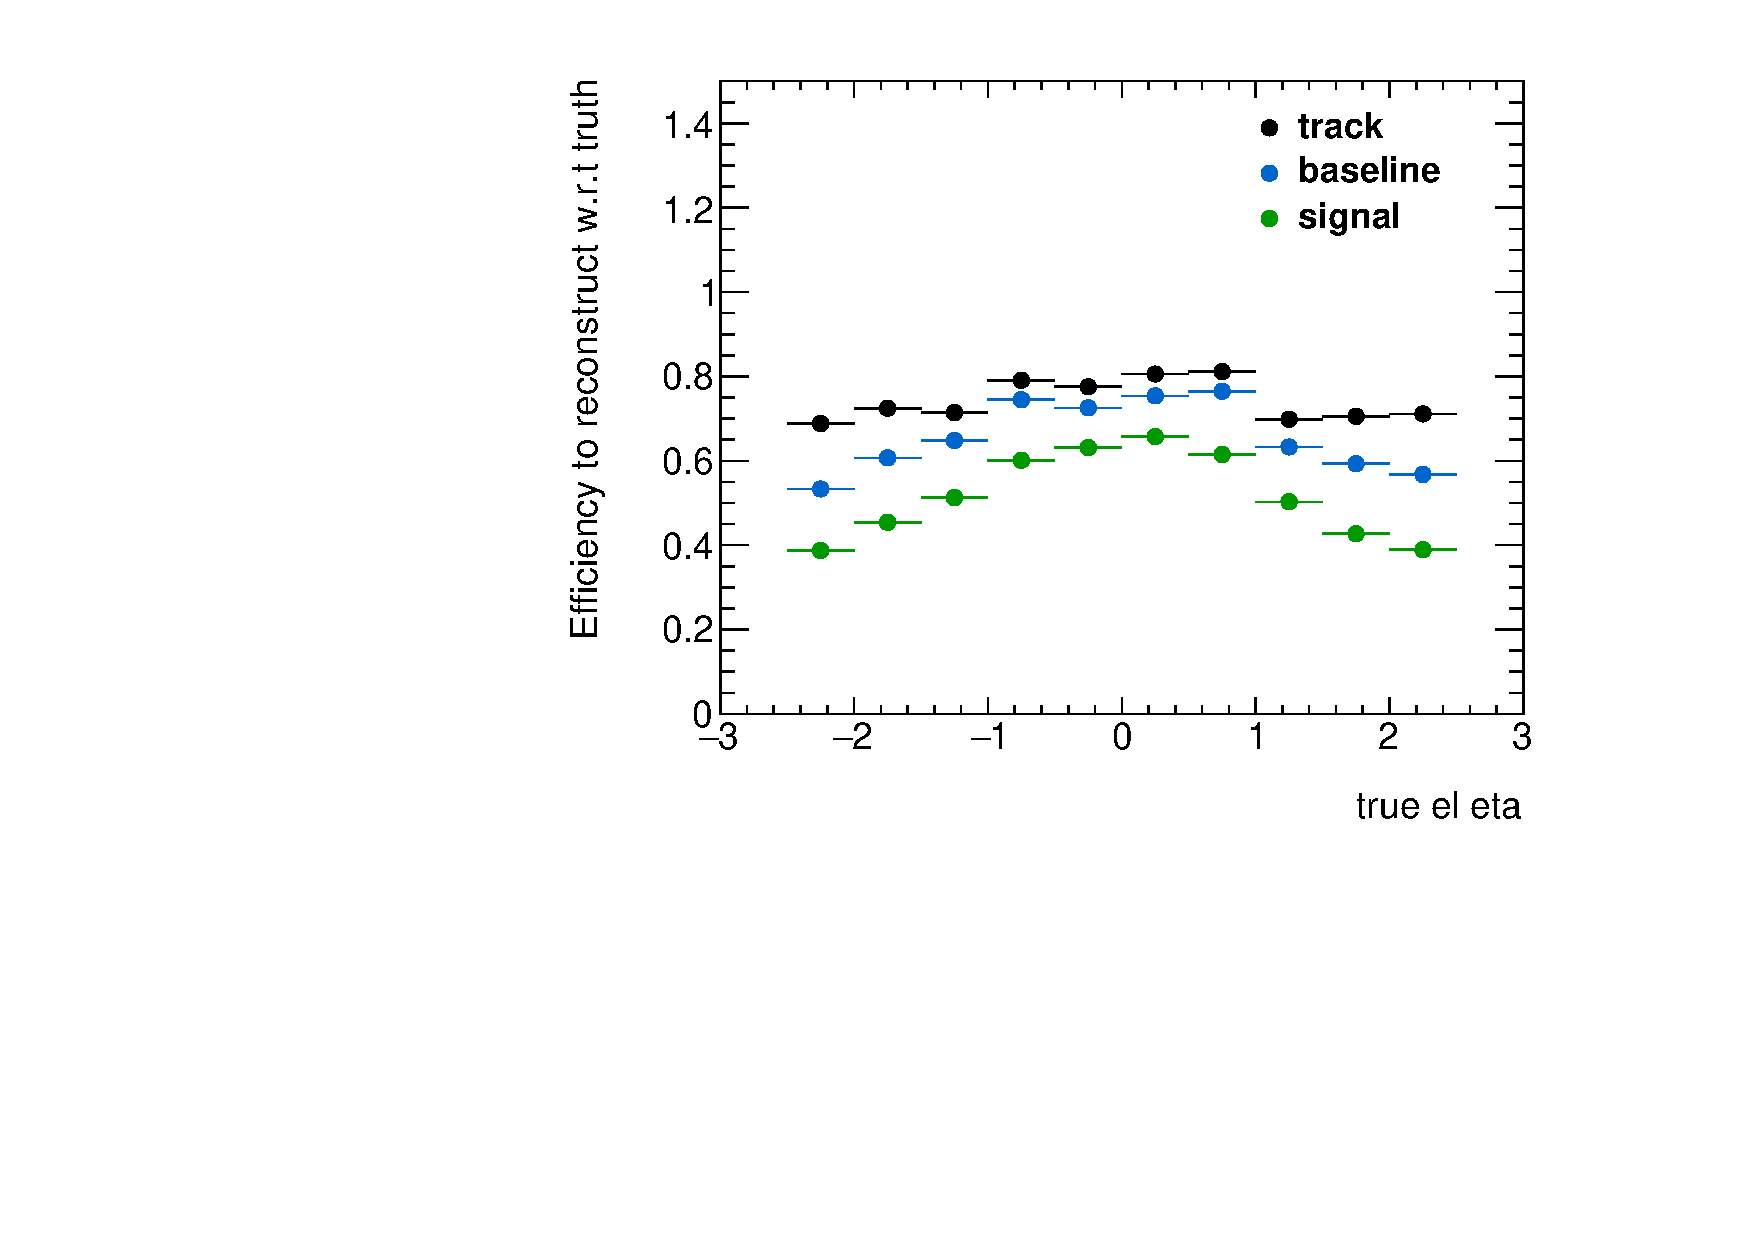
\includegraphics[width=.48\textwidth]{figures/disp_systs/signal_effcompare_eta_el_300.pdf}
%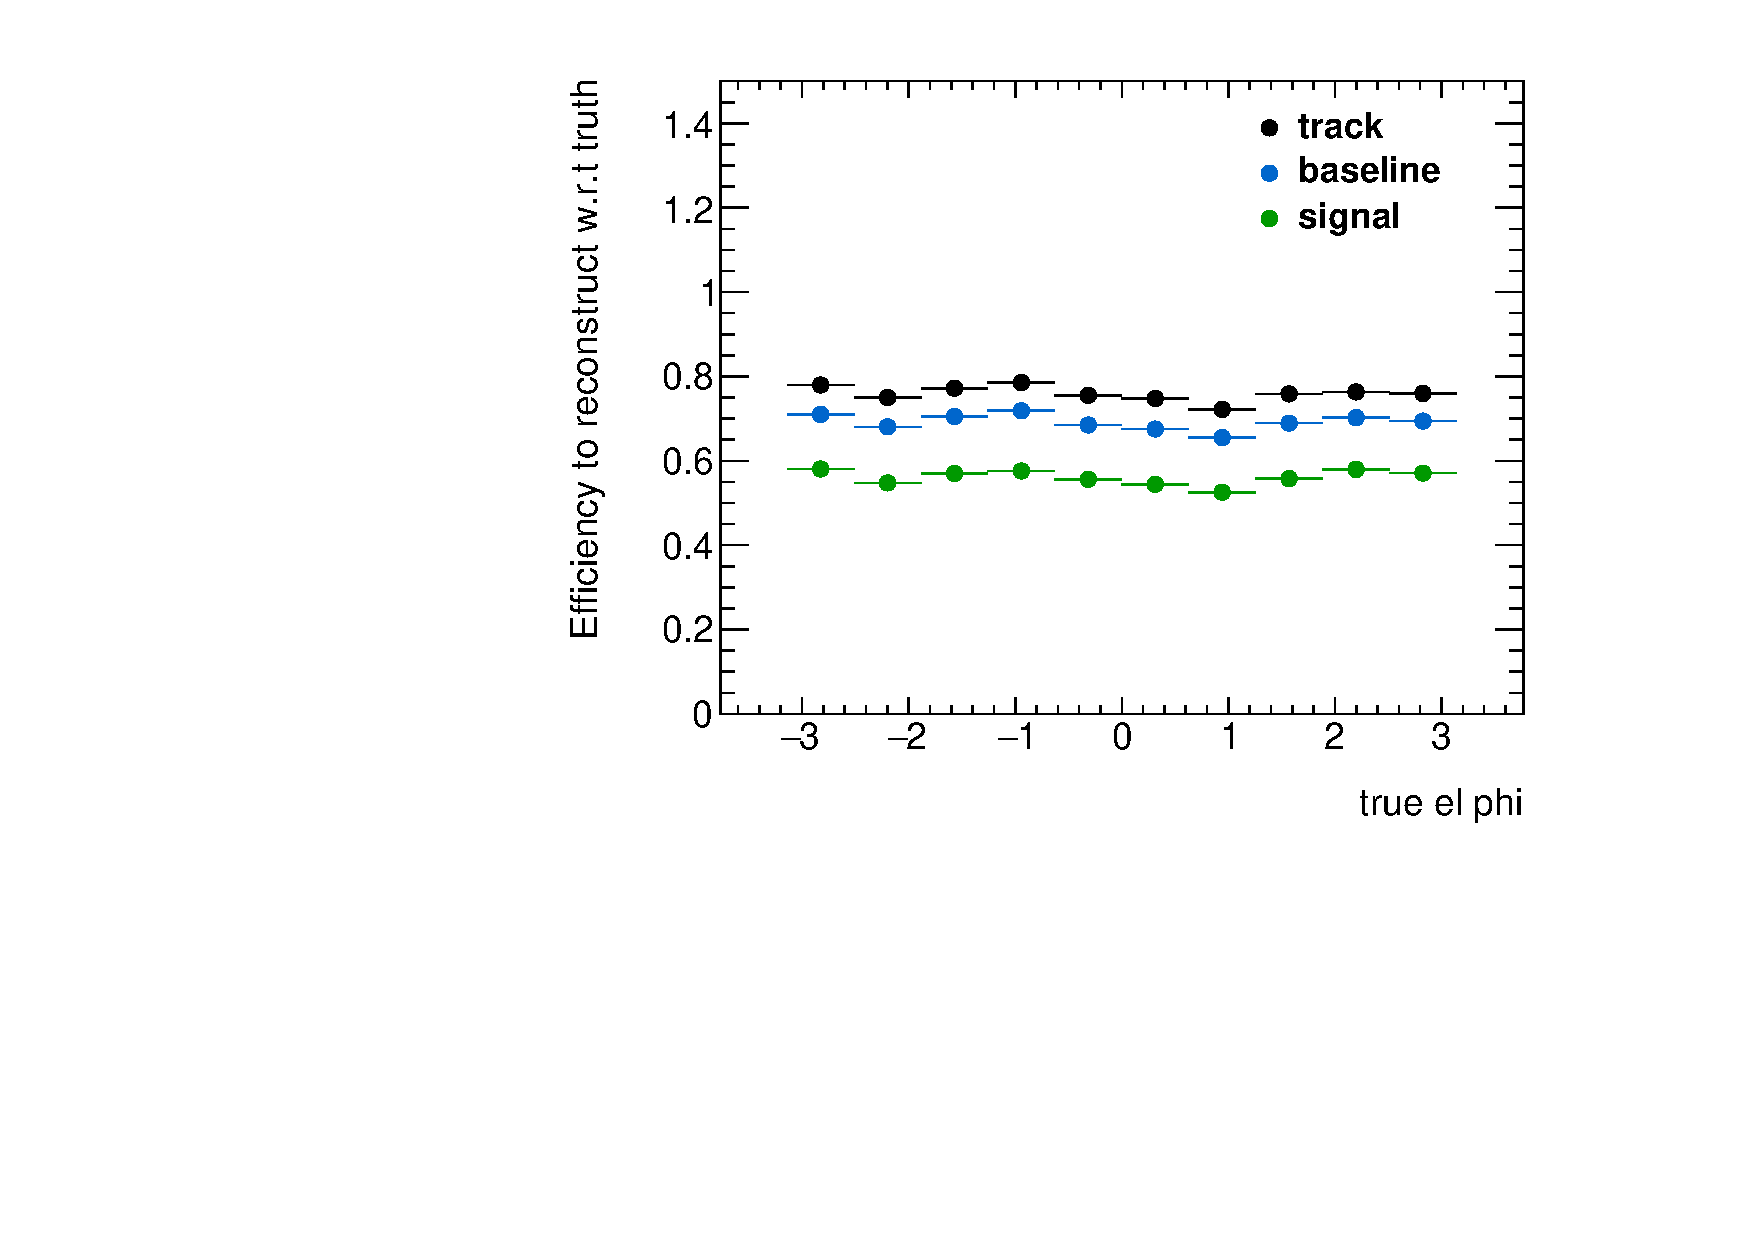
\includegraphics[width=.48\textwidth]{figures/disp_systs/signal_effcompare_phi_el_300.pdf}
%\caption{Electron selection efficiencies vs $R_{\textrm{decay}}$ (top left), \pt (top right), $\eta$ (bottom left), and $\phi$ (bottom right). Plots are made from 300 GeV slepton signal samples with lifetimes between 0.01-1ns. The denominator of the efficiency is truth muons from sleptons with \pt > 65 GeV and $|\eta|$ < 2.5, and the numerator is truth matched and signal (or baseline) quality tracks or leptons.}
%\label{fig:effs_el}
%\end{figure}

%\begin{figure}[htbp]
%\centering
%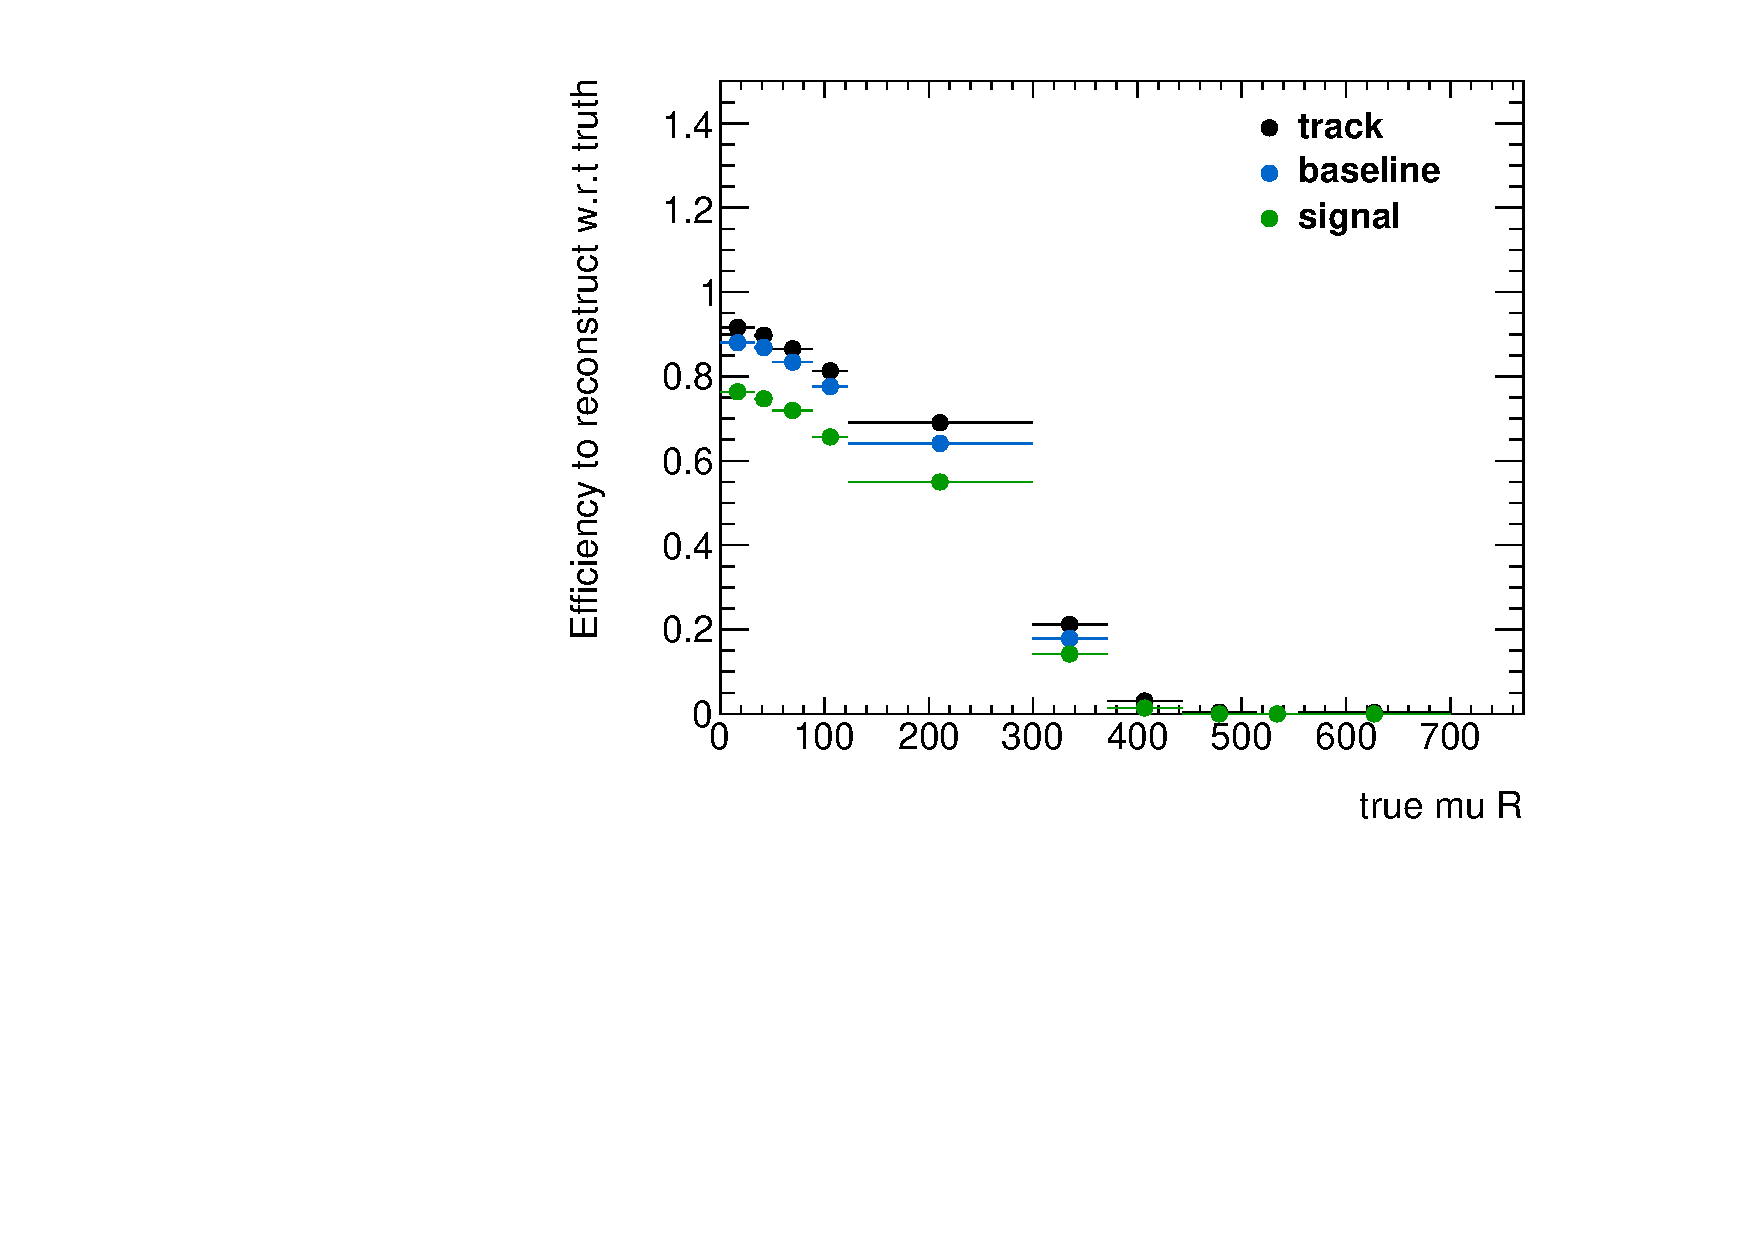
\includegraphics[width=.48\textwidth]{figures/disp_systs/signal_effcompare_R_mu_300.pdf}
%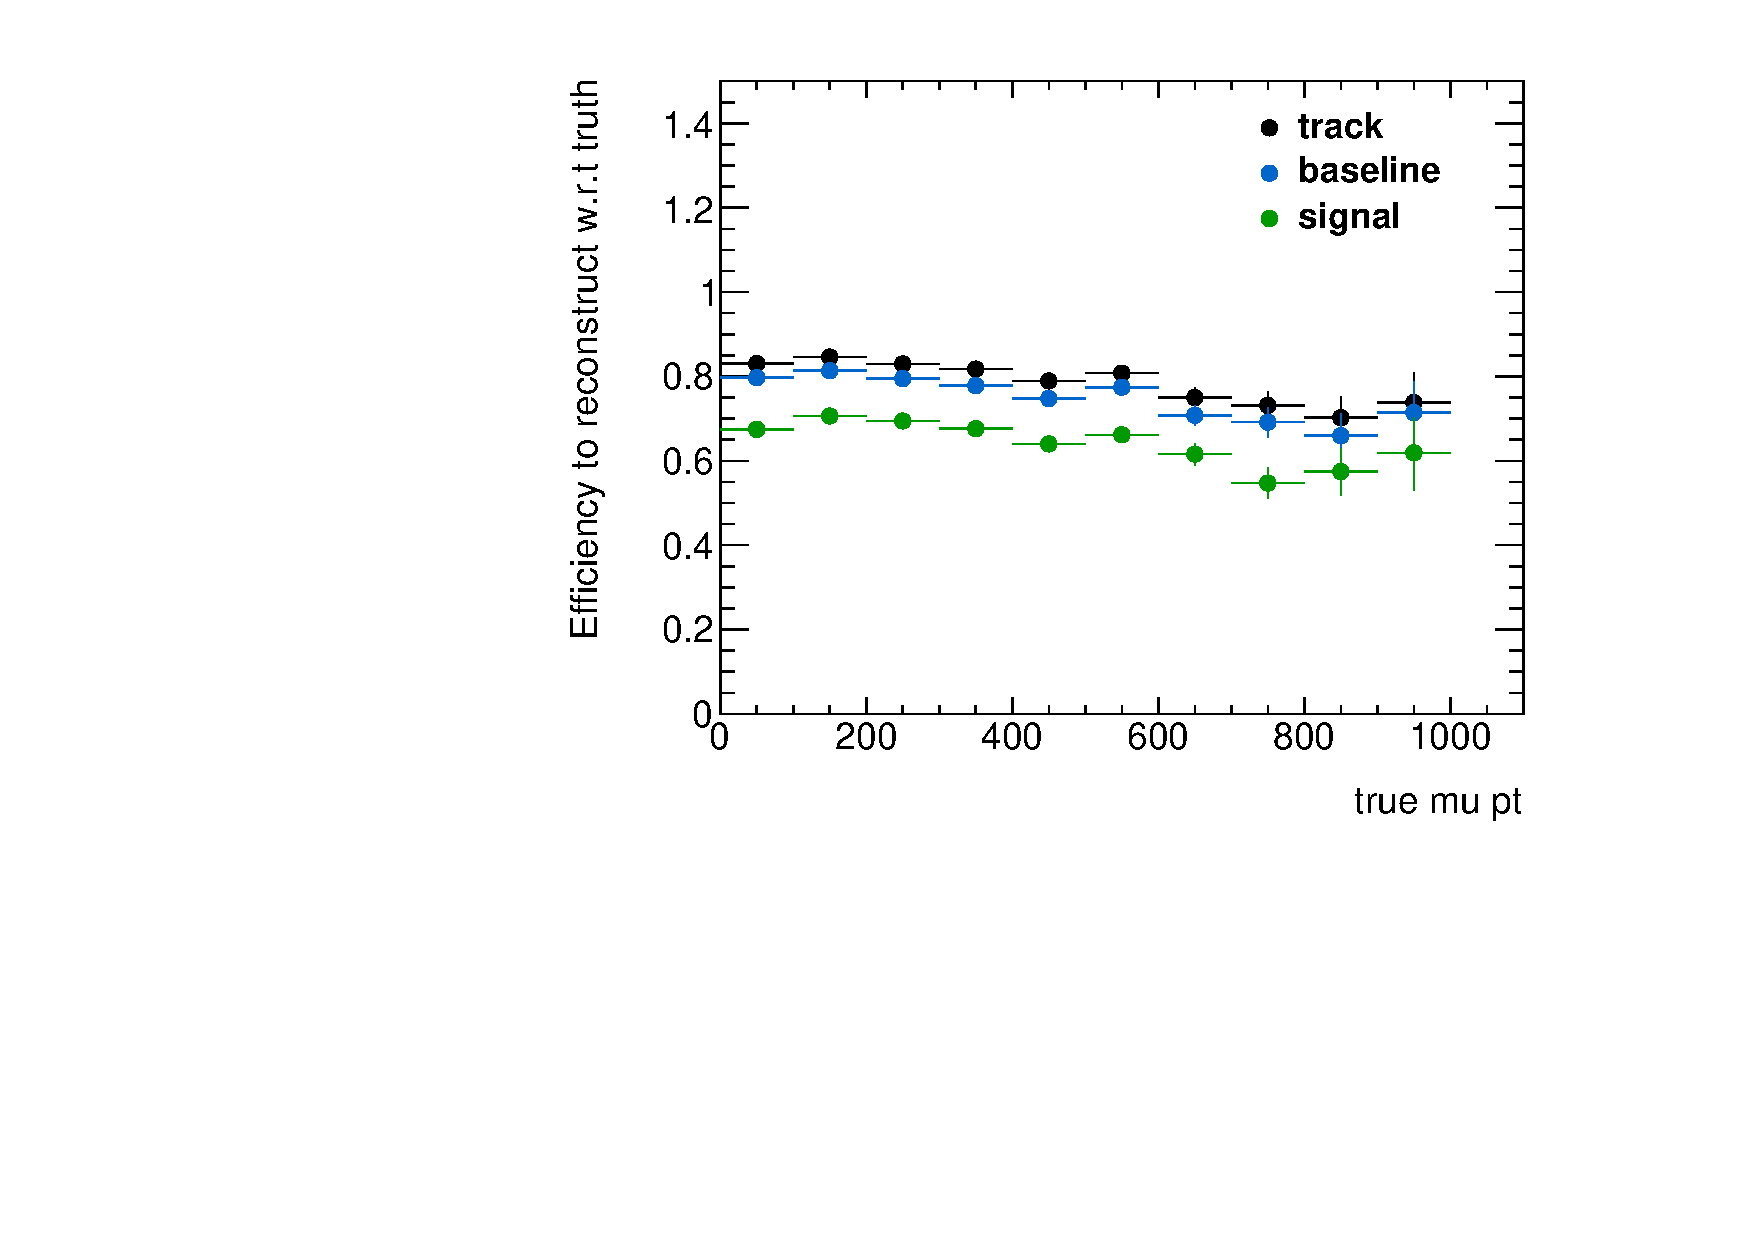
\includegraphics[width=.48\textwidth]{figures/disp_systs/signal_effcompare_pt_mu_300.pdf}
%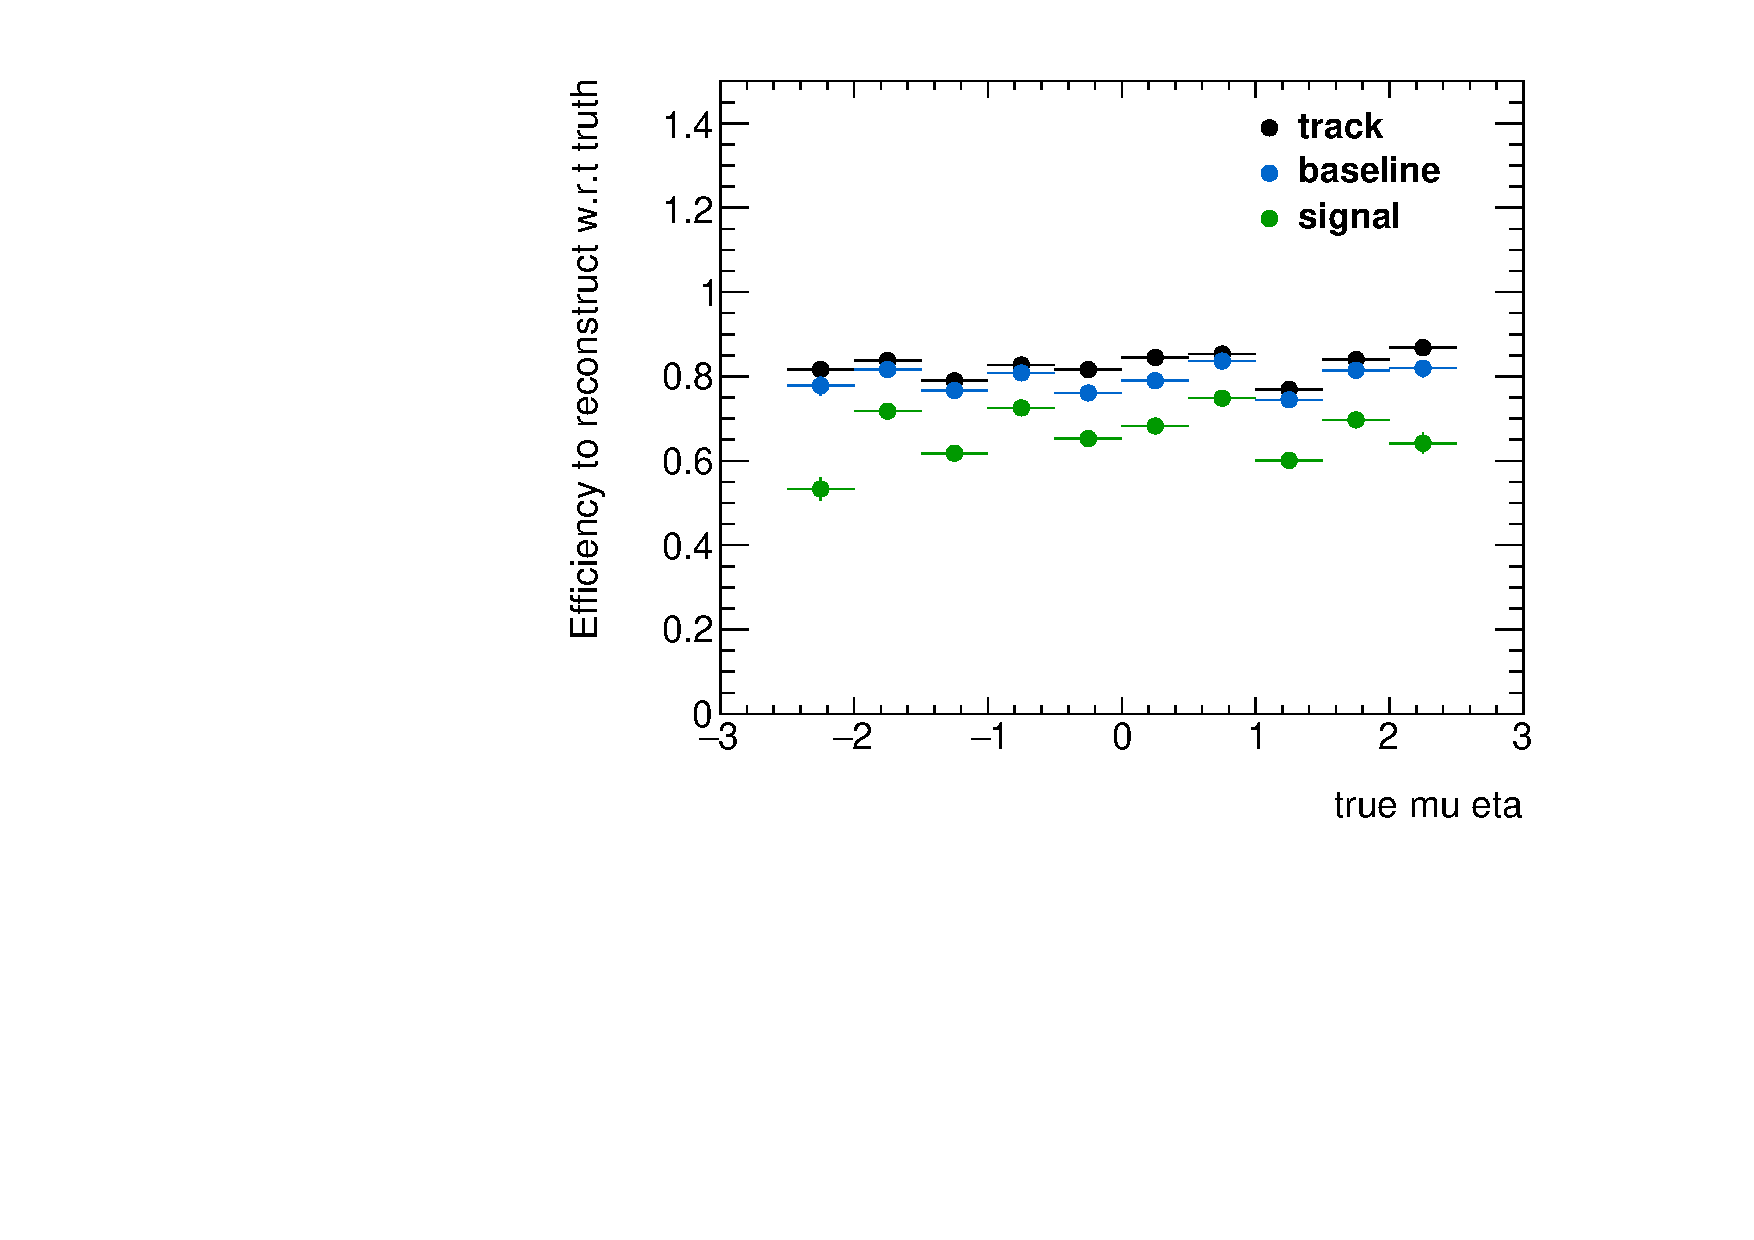
\includegraphics[width=.48\textwidth]{figures/disp_systs/signal_effcompare_eta_mu_300.pdf}
%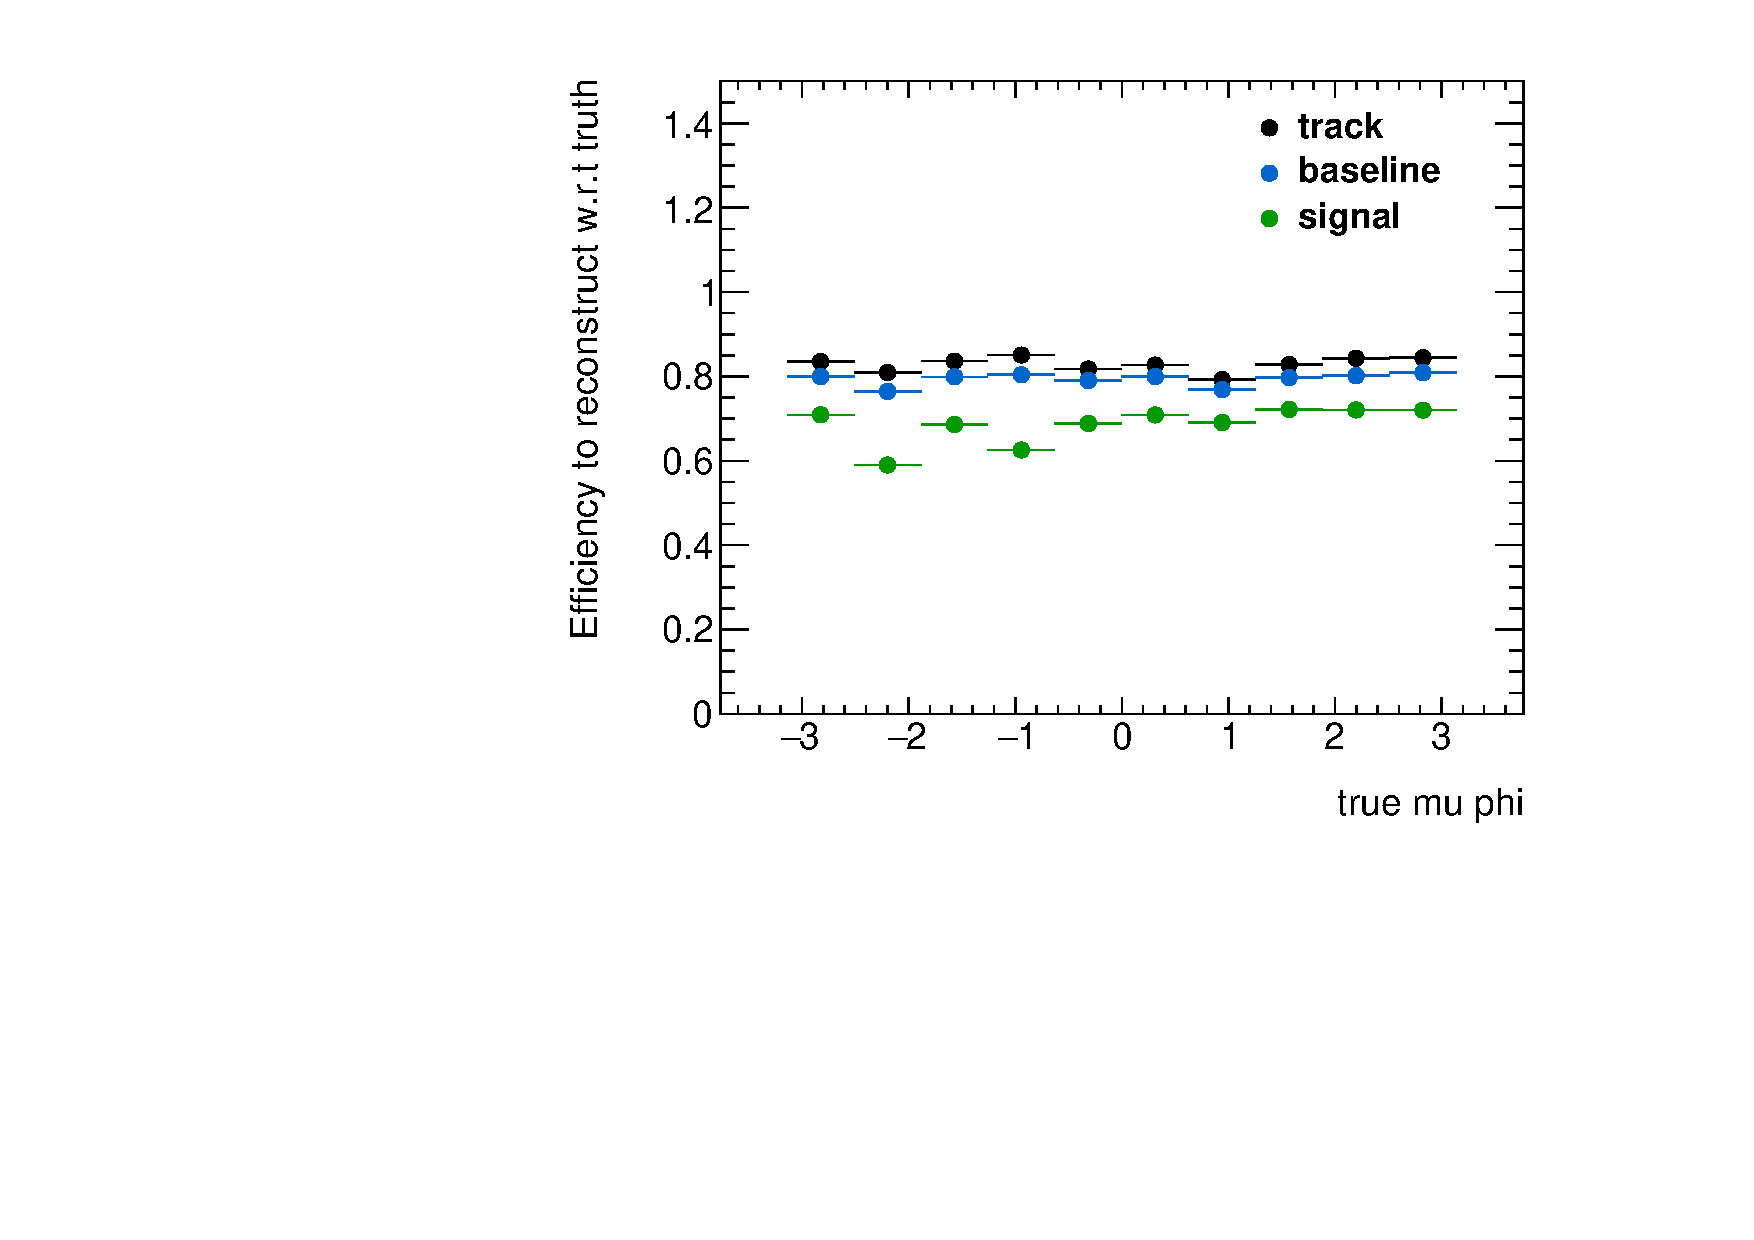
\includegraphics[width=.48\textwidth]{figures/disp_systs/signal_effcompare_phi_mu_300.pdf}
%\caption{Electron selection efficiencies vs $R_{\textrm{decay}}$ (top left), \pt (top right), $\eta$ (bottom left), and $\phi$ (bottom right). Plots are made from 300 GeV slepton signal samples with lifetimes between 0.01-1ns. The denominator of the efficiency is truth muons from sleptons with \pt > 65 GeV and $|\eta|$ < 2.5, and the numerator is truth matched and signal (or baseline) quality tracks or leptons.}
%\label{fig:effs_mu}
%\end{figure}



%Small trends in \dz can be seen in some shower shape variables, particularly in ERatio and RHad, though not enough to explain the full discrepancy from the prompt efficiency. In muons, trends can be seen in the \ac{MS} track $\chi^{2}$ as well as the Eloss, and in electrons trends can be seen in $f_{1}$ and ERatio. We checked for, but did not find, trends in \dz with respect to other \ac{MS} track or shower shape variables. 


%\begin{figure}[htbp]
%\centering
%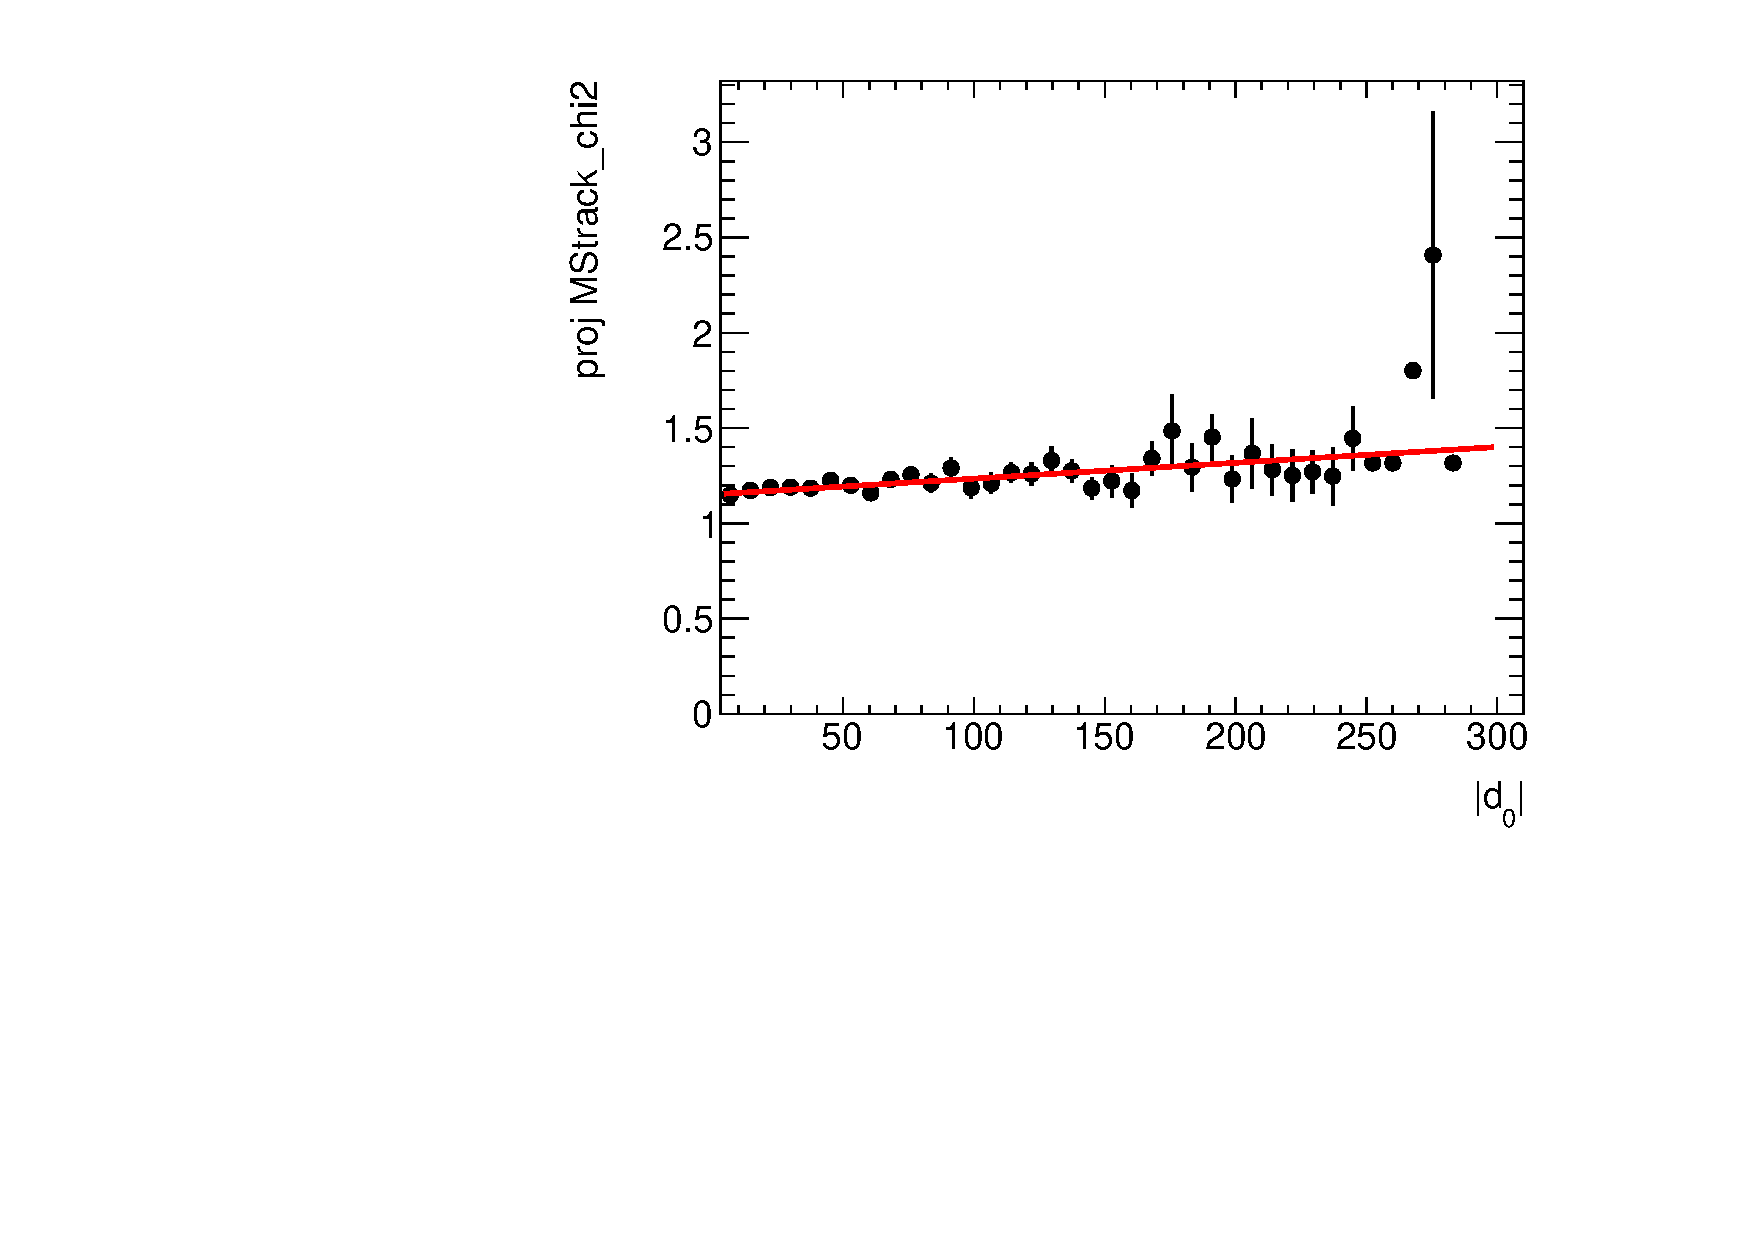
\includegraphics[width=.48\textwidth]{figures/disp_systs/m_signal_MStrack_chi2_profile.pdf}
%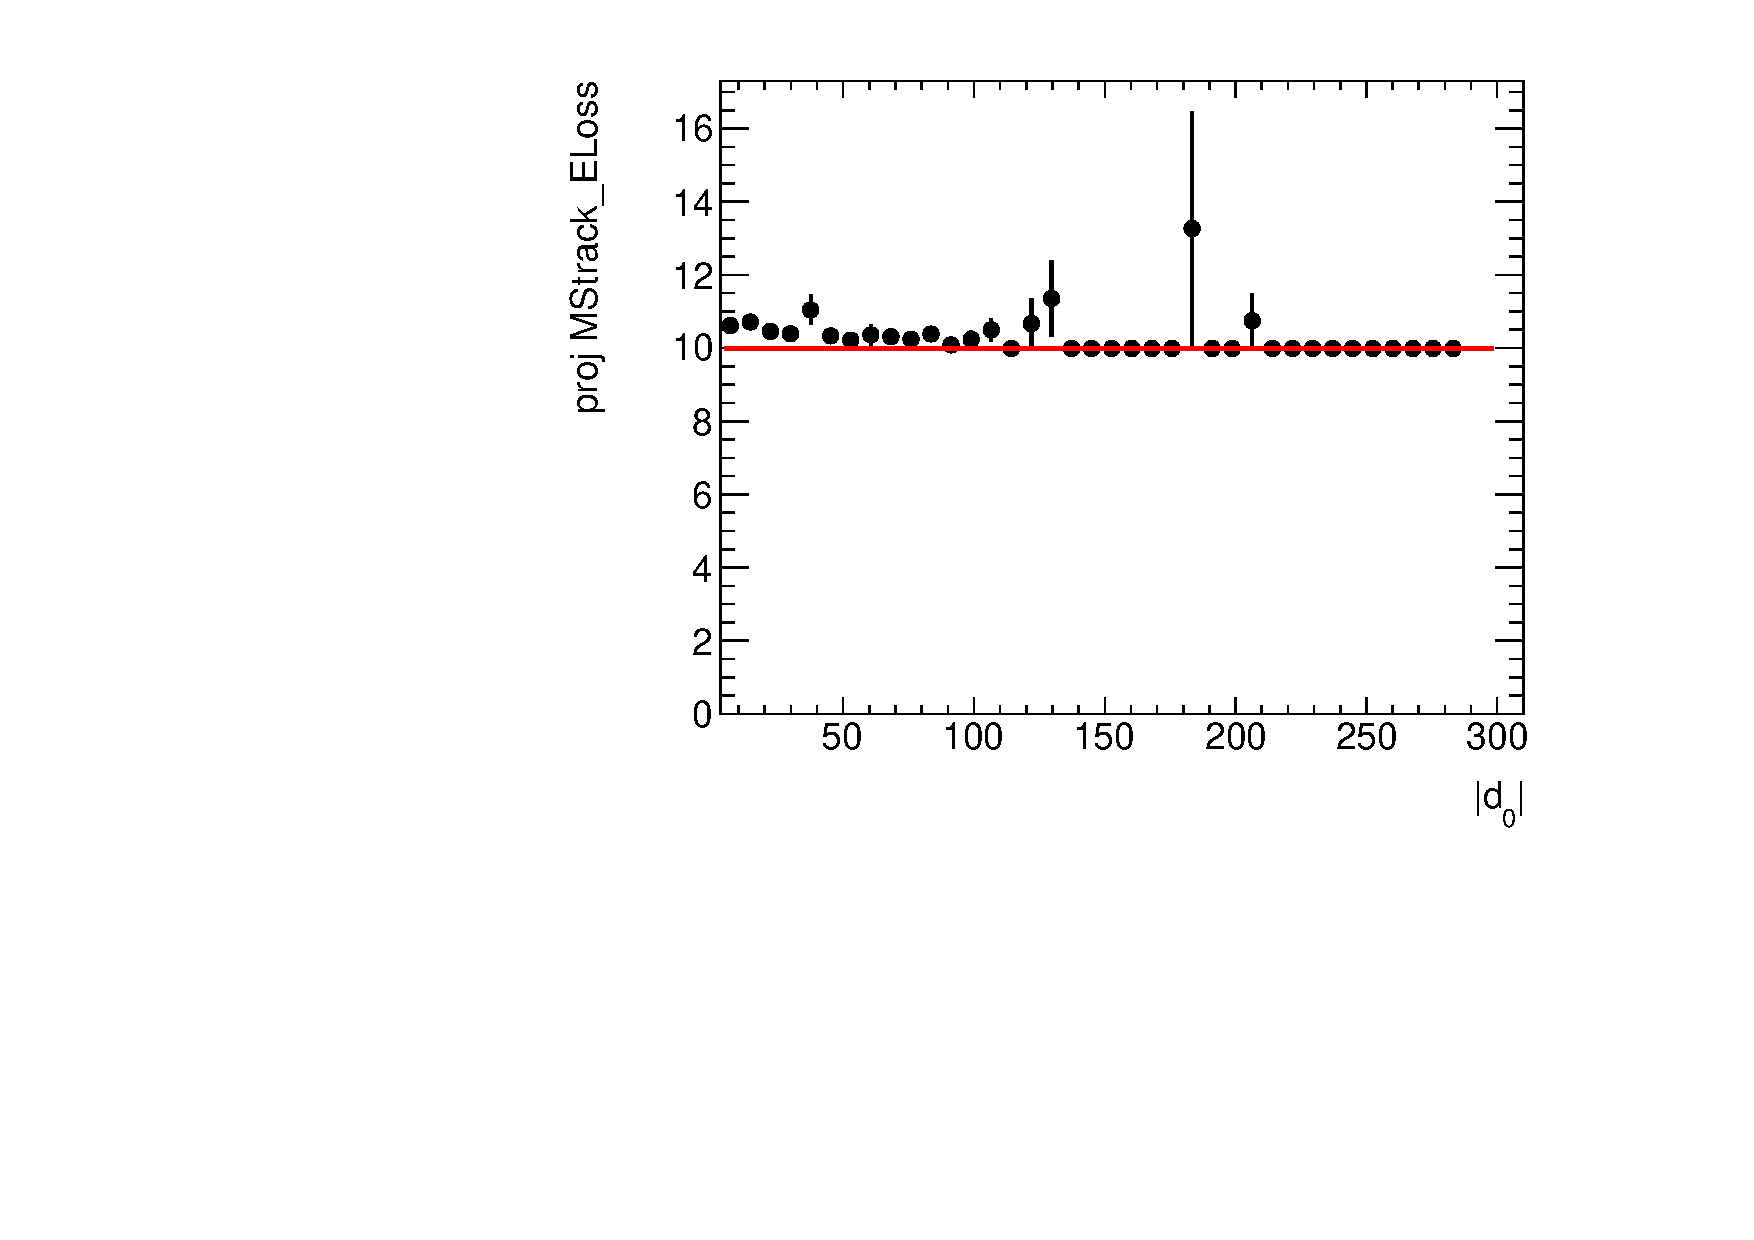
\includegraphics[width=.48\textwidth]{figures/disp_systs/m_signal_MStrack_ELoss_profile.pdf}
%\caption{Muon quality variables with trends with respect to \absdz, \ac{MS} track $\chi^{2}$ (left) and Eloss. Taken from a 300 GeV signal sample with lifetimes between 0.01ns-1ns.}
%\label{fig:profs_mu}
%\end{figure}

%\begin{figure}[htbp]
%\centering
%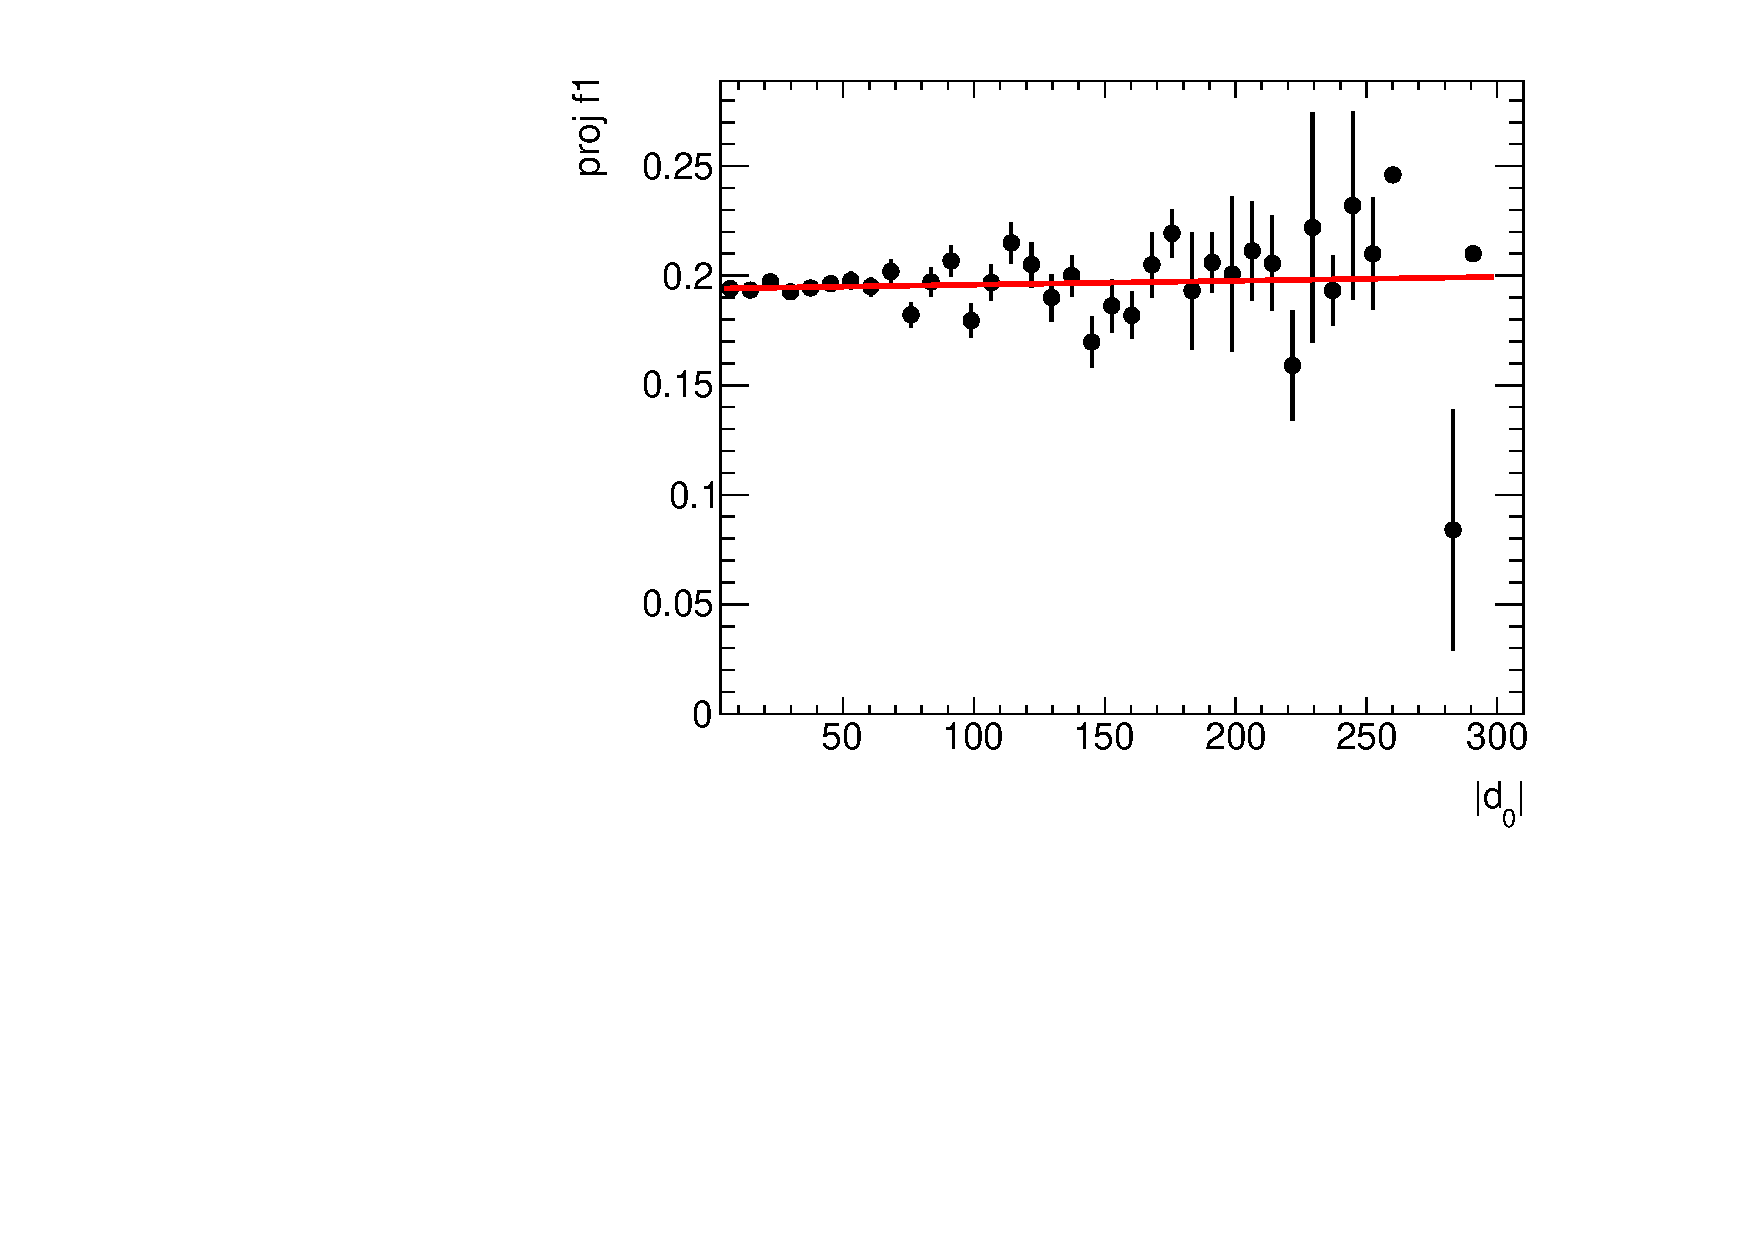
\includegraphics[width=.48\textwidth]{figures/disp_systs/e_signal_f1_profile.pdf}
%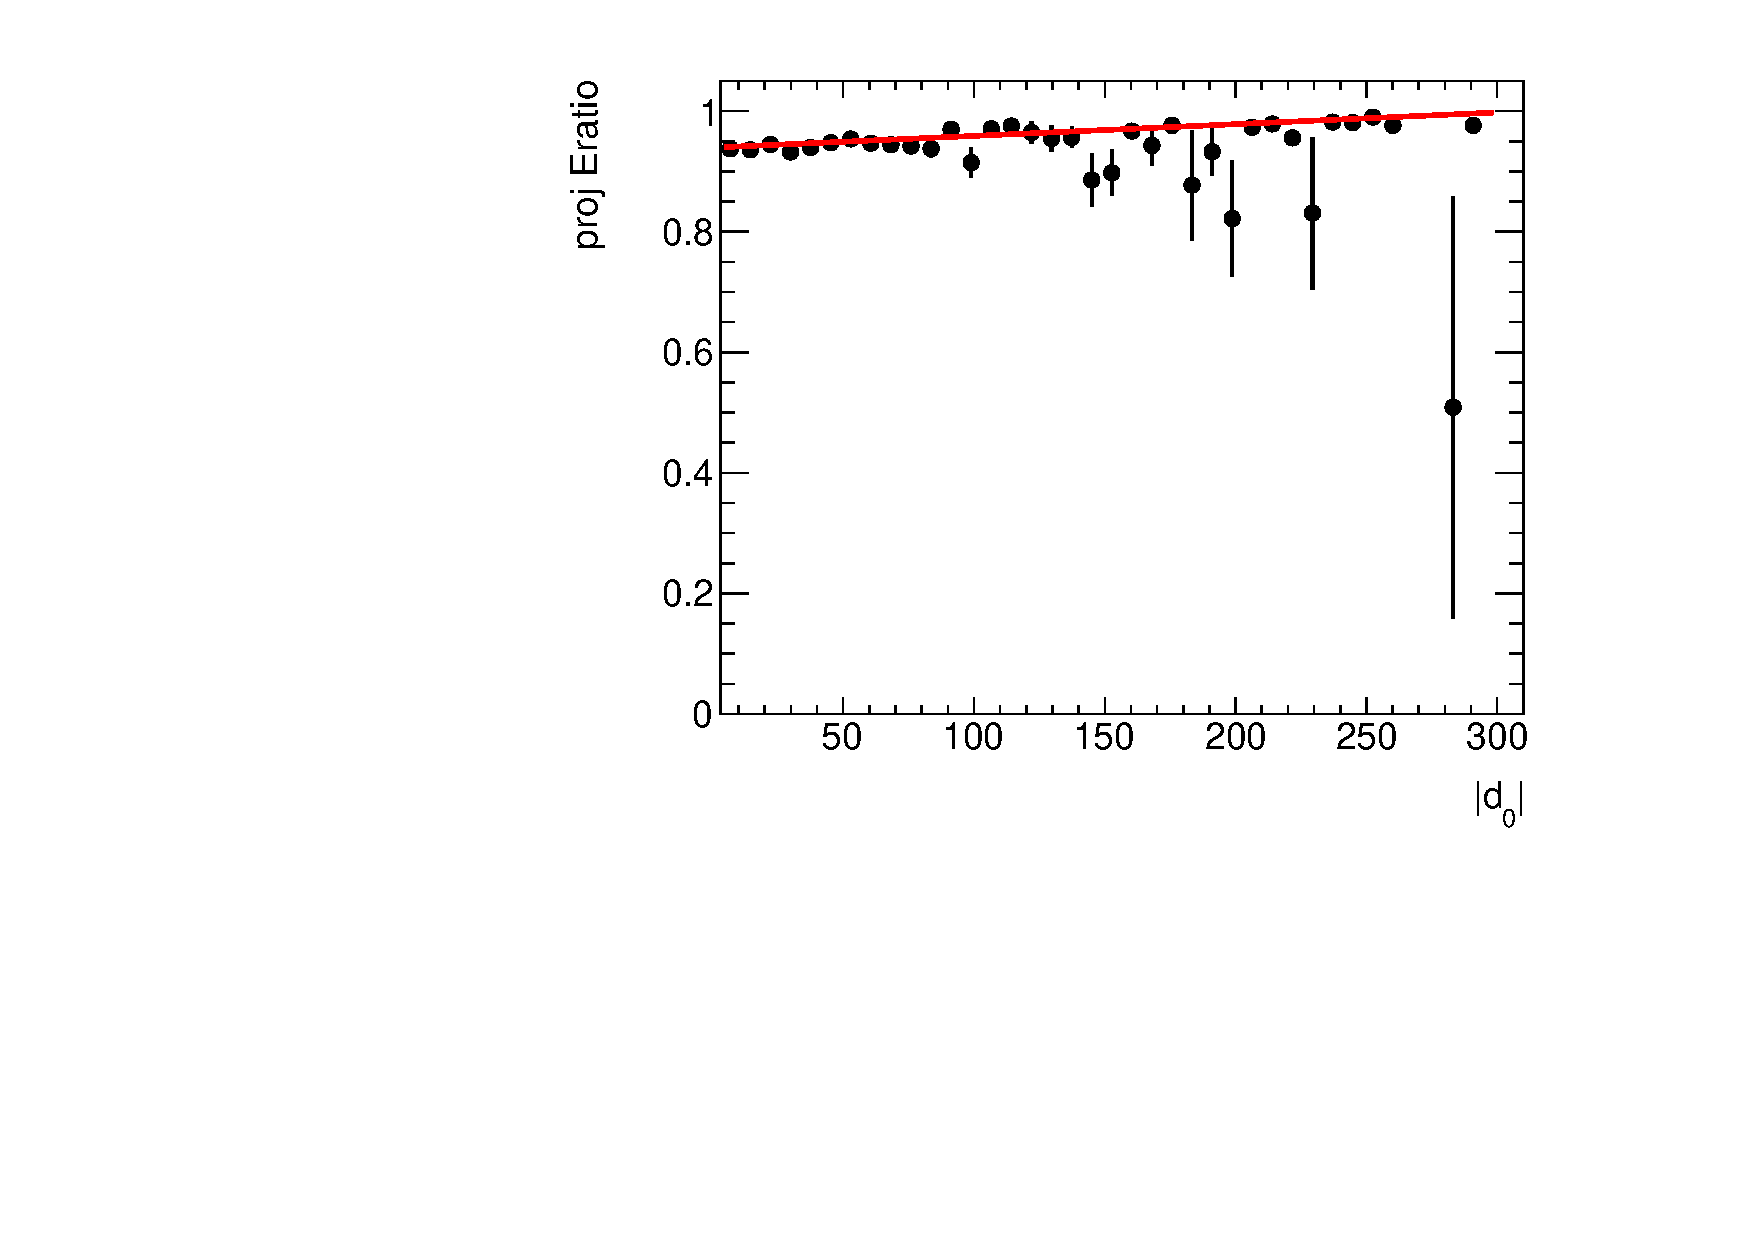
\includegraphics[width=.48\textwidth]{figures/disp_systs/e_signal_Eratio_profile.pdf}
%\caption{Electron shower shape quality variables with trends with respect to \absdz, $f_{1}$ (left) and ERatio. Taken from a 300 GeV signal sample with lifetimes between 0.01ns-1ns.}
%\label{fig:profs_el}
%\end{figure}


\subsection{Other Sources of Uncertainty}

\subsubsection{Pileup Modeling}
When \ac{MC} is generated, particularly when it is generated during the course of the run, the actual pileup distribution of the events from the \ac{LHC} is not known. This is corrected through a process called \emph{pileup reweighting}, where a more realistic pileup profile is added to \ac{MC} events. The change in number of signal events when the pileup profile is varied is taken as a systematic uncertainty, 2\%.

\subsubsection{Theoretical Uncertainties}

Additional uncertainties are taken for the renormalization and factorization scales that are used to generate the physical processes in \ac{MC}. These impact both the cross section measurement and the final lepton kinematics. Both scales are varied, impact on the final results quantified, and the range of variation is taken as an uncertainty, in this analysis about 5\%. 

\subsubsection{Luminosity Measurement}
\ac{ATLAS} measures luminosity using dedicated detectors and calibrations (discussed in \autoref{sec:lumi}. The uncertainty on this measurement contributes a 2\% uncertainty to the analysis, as it impacts the normalization of the signal yield from \ac{MC}.




